\documentclass[12pt]{report}

% Use UTF-8 encoding for the document
\usepackage[utf8]{inputenc}

% Use german language
\usepackage[german]{babel}

% Use Times as font family for the document
\usepackage[T1]{fontenc}

\usepackage{hyperref}

% Set line height to 1.5
\renewcommand{\baselinestretch}{1.5}

% Set spacing of the outer edges of the page
\usepackage{geometry}
\geometry{a4paper, top=20mm, left=30mm, right=20mm, bottom=30mm, footskip=15mm}

% Set header and footer
\usepackage{fancyhdr}
\pagestyle{fancy}
\fancyhead{}
\renewcommand{\headrulewidth}{0pt}
\cfoot{} % Surpress centered line number
\rfoot{\thepage}

% For incluing graphics
\usepackage{graphicx}

% For name references
\usepackage{nameref}

% Code listings
\usepackage{listings}

% Don't indent paragraphs
\usepackage{parskip}

% Enable usage of urls
\usepackage{url}

\usepackage{xcolor}
\usepackage{textcomp}

\usepackage{inconsolata}



% Inlcude subsubsection in ToC
\setcounter{tocdepth}{4}
\setcounter{secnumdepth}{4}

% Define styles for JS language
\definecolor{lightgray}{rgb}{.9,.9,.9}
\definecolor{darkgray}{rgb}{.4,.4,.4}
\definecolor{purple}{rgb}{0.65, 0.12, 0.82}

\lstdefinelanguage{JavaScript}{
  keywords={typeof, new, true, false, catch, function, return, null, catch, switch, var, if, in, while, do, else, case, break},
  keywordstyle=\color{blue}\bfseries,
  ndkeywords={class, export, boolean, throw, implements, import, this},
  ndkeywordstyle=\color{darkgray}\bfseries,
  identifierstyle=\color{black},
  sensitive=false,
  comment=[l]{//},
  morecomment=[s]{/*}{*/},
  commentstyle=\color{purple}\ttfamily,
  stringstyle=\color{red}\ttfamily,
  morestring=[b]',
  morestring=[b]"
}

% lstlisting styles
\lstset{
   language=JavaScript,
   backgroundcolor=\color{white},
   extendedchars=true,
   basicstyle=\scriptsize\ttfamily,
   lineskip={0.5pt},
   showstringspaces=false,
   showspaces=false,
   numbers=left,
   numberstyle=\scriptsize\ttfamily,
   numbersep=9pt,
   tabsize=2,
   breaklines=true,
   showtabs=false,
   captionpos=t,
   frame=single
}


\begin{document}
\begin{titlepage}

\begin{center}

% Logo der Technische Hochschule Köln
% Kann auch in dieser Form in Schwarz/Weiß ausgedruckt werden; Graustufen sollten der .tif Version entsprechen
\begin{flushleft}

\includegraphics[width=0.26\textwidth]{images/logo_th.jpg}
\end{flushleft}

\vspace{1.6cm}

%Deutscher Titel
{\Large\textbf{25knots – Ein Tool zur Verbesserung der gestalterischen Qualität von Artefakten im Hochschulkontext}\par}
\vspace{0.5cm}
\begin{large}
Umsetzung vom Proof of Concept zur marktfähigen Webanwendung
\end{large}

\vspace{1.2cm}

%Bachelorarbeit
\begin{LARGE}
\begin{scshape}
Bachelorarbeit\\
\end{scshape}
\end{LARGE}

\vspace{0.8cm}

\begin{normalsize}
vorgelegt an der Technischen Hochschule Köln\\
Campus Gummersbach\\
im Studiengang Medieninformatik\\
\end{normalsize}
\vspace{0.8cm}

%ausgearbeitet von...
ausgearbeitet von\\
\vspace{0.2cm}
\begin{large}
Christian Alexander Poplawski, 11088931\\
\end{large}

\vspace{1.6cm}

%Autor der Bachelorarbeit und die Prüfer
\begin{tabular}{rl}
        Erster Prüfer:  &  Prof. Dipl. Des. Christian Noss\\
       					&  \small Technische Hochschule Köln \\[1.0em]
       Zweiter Prüfer:  &  Dipl. Des. Liane Kirschner\\
       					&  \small Railslove GmbH\\
\end{tabular}

\vspace{1.6cm}

%Ort, Monat der Abgabe
\begin{large}
Gummersbach, im August \the\year
\end{large}

\end{center}

\end{titlepage}

\tableofcontents

\listoffigures

\chapter{Einleitung}
\thispagestyle{fancy}
Thema der Abschlussarbeit soll die Umsetzung und Gestaltung einer Webanwendung auf Basis von bereits im Praxisprojekt erarbeiteten Konzepten sein.
Die Anwendung hat das Ziel, ihren Nutzern dabei zu helfen, in der Gestaltung von Artefakten eine Grundqualität zu sichern. Die Konzepte wurden speziell auf Studenten des Studiengangs Medieninformatik an der TH Köln ausgelegt, die auch die primäre Zielgruppe der Anwendung sein sollen. Die Festlegung auf diese Zielgruppe schließt aber auch andere Nutzer nicht aus, im weitesten Sinne kann die Anwendung für jede Person hilfreich sein, die die Gestaltung eines Artefaktes verbessern möchte, aber nicht über das nötige Wissen verfügt.\\

\section{Motivation}
Im Rahmen des Praxisprojektes wurden einige grundlegende Konzepte zu einer Anwendung erarbeitet, wie sie in der Abschlussarbeit erstellt werden soll. Die Motivation für die Umsetzung rührt daher, dass die Ergebnisse des Praxisprojektes nicht nur auf dem Papier zum Erlangen von Credit Points dienen sollen, sondern meiner Meinung nach auch tatsächlich im Arbeitsalltag von Nutzen hilfreich sein können. Diese Ansicht unterstützen Gespräche, die mit Personen verschiedener Professionen (zum Beispiel Designer und Entwickler) geführt wurden und während derer sich eine Nachfrage nach einen solchen Produkt durchaus erkennen ließ.

\section{Zielsetzung}
Ziel der Abschlussarbeit soll es sein, ein verwendbares Produkt zu erstellen. \textit{Verwendbar} lässt sich hierbei in drei Unterzielen definieren:

\begin{enumerate}
  \item Die Anwendung muss einen hohe Qualität aufweisen, um eine befriedigende Nutzererfahrung zu bieten
  \item Die Anwenung muss öffentlich zugänglich sein
  \item Potentielle Nutzer müssen von der Existenz der Anwendung wissen
\end{enumerate}

Das Hauptaugenmerk der Arbeit wird dabei auf der sicherung der Qualität das Produktes liegen. Hier spielen sowohl die Programmierung der Anwendung, als auch das Design (Visuell und Strukturell) eine Schlüsselrolle. \\
Um die Anwendung öffentlich zugänglich zu machen muss eine Entscheidung über das Hosting getroffen werden. Dabei soll der Dienst \textit{Heroku} verwendet werden. Dieser bietet die Möglichkeit, ohne übermäßige Konfiguration Inhalte zu hosten und lässt sich nach Bedarf erweitern, um beispielsweise höhere Nutzerzahlen abbilden zu können. \\
Damit potentielle Nutzer Kenntnis von der Anwendung erhalten, muss diese beworben werden. Mit Blick auf die Zielgruppe bietet sich zunächst eine Bewerbung direkt an der Hochschule, beispielweise durch die Teilnahme am \textit{Medieninfromatik Showcase} an. Aber auch eine Bewerbung im weiteren Rahmen, beispielsweise durch einen Talk beim \textit{Webmontag Köln} ist denkbar.

Zuletzt soll auch eine mögliche spätere Weiterentwicklung der Anwendung bedacht werden, denn im Rahmen der Abschlussarbeit können unmöglich alle für die Gestaltung wichtigen Themen abgedeck werden. Der Quellcode der Anwendung soll auf der Plattform \textit{Github} öffentlich zur Verfügung stehen, so dass auch Dritte an der Weiterentwicklung beteiligt sein können. Mit Blick auf die Beiteiligung dritter muss es auch Ziel der Arbeit sein, den Quellcode gut zu strukturieren und dokumentieren, um einen Einsteig für neue Personen möglichst einfach zu machen.

\section{Relevanz des Themas}
BDie Relevanz der Anwendung an sich wurde bereits im Praxisprojekt erläutert, daher soll hier nur eine Kurzfassung der Erläuterung folgen:\\
Lindgaard et al. \cite{lindgaard2006attention} haben gezeigt, dass Menschen sich in nur 50ms ein Urteil über die Gestaltung einer Website bilden. Der erste Eindruck spielt bei Menschen auch bei der späteren Bewertung einer Sache noch eine wichtige Rolle \cite{campbell1996fitting}. Von diesem ersten Eindruck lassen sich Menschen nur schwer wieder abbringen \cite{nickerson1998confirmation}.
Daher ist es wichtig, dass auch Artefakte in Modulen, in denen die Gestaltung gegebenenfalls nicht bewertet wird, ein solides Design aufweisen, um den ersten Eindruck so positiv wie möglich zu gestalten.

Unterstützend seien hier noch zwei weitere Quellen aufgeführt, die die Relevanz weiter unterstreichen:\\
\cite{tractinsky2006evaluating} zeigen, dass die Ergebnisse der Studie von Lindgaard et al. auch mit anderen Parametern bestand haben und unterstreichen weiterhin die Wichtigkeit von guter Gestaltung für eine gute Nutzererfahrung \cite{tractinsky2000beautiful}.\\
Auch aus vielen persönlichen Gespräche konnte ich entnehmen, dass die Umsetzung der erarbeiteten Konzepte als Produkt, auch für verschiedene Personengruppen, durchaus wünschenswert ist.

Neben der Relevanz des Produktes, das in Rahmen der Arbeit entstehen soll ist aber auch das eigentliche Thema der Arbeit zu rechtfertigen: Die Entwicklung von einem Konzept zu einem fertigen Produkt.
Als abschließende Arbeit für den Studiengang Medieninformatik ist dies ein passendes Thema, da in diesem viele Aspekte des gesamten Studiums vereint werden. In den weiter oben genannten Bereichen kommen beispielsweise Inhalte aus den Modulen GdvK, WBA 1, ST,  PM und EIS vor. Daher bietet das Thema eine gute Verbindung zwischen den verschiedenen Disziplinen innerhalb des Studiums, verbunden mit einer wissenschaftlichen Diskussion verschiedener Vorgehensweisen und Abläufe.

\section{Abgrenzung}
Bei der Textgestaltung und automatischen Änderung von Abbildungsnummern, Querverweisen,
Seitenzahlen, Gliederungen, Literaturhinweisen etc. bietet sich der Rückgriff
auf moderne Textverarbeitungsprogramme an. Nutzen Sie diese zur besseren Lesbarkeit
und Strukturierung des Textes, aber vermeiden Sie überflüssige Spielereien. Da
besonders bei Textdokumenten mit eingebundenen Objekten wie Bildern, Formeln

\section{Struktur der vorliegenden Arbeit}
asdf
asd
asd

asd
asd
asd

\chapter{Konzeption der Anwendung}
\thispagestyle{fancy}

\section{Generelle Struktur der Anwendung}
Zu Beginn gilt es, die verschiedenen Bereiche der Gestaltung zu definieren, die die fertiggestellte Anwendung behandeln soll. Innerhalb des Praxisprojektes wurden verschiedene Themengebiete behandelt, die an dieser Stelle erneut auf eine Umsetzbarkeit hin validiert werden müssen. Die im Praxisprojekt definierten Themengebiete sind:

\begin{itemize}
  \item Typographie
  \item Layout \& Struktur
  \item Whitespace
  \item Farben
  \item Bilder
  \item Interaktive Elemente
\end{itemize}

Der Bereich \textit{Whitespace} konnte schnell ausgeschlossen werden, da obgleich seiner Wichtigkeit für eine gute Gestaltung währen des Praxisprojektes keine Konzepte gefunden werden konnten, auf deren Basis eine Umsetzung möglich wäre.\\
Vor der Zielsetzung, nach Abschluss der Arbeit eine Marktfähige (und damit in ihren Features vollständige) Anwendung erstellt zu haben und der gegebenen Zeit von 9 Wochen für die Umsetzung dieser, musste die Liste der zu behandelnden Gebiete noch weiter eingeschränkt werden.\\
Hier wurde sich für die Bereiche \textit{Bilder} und \textit{Interaktive Elemente} entschieden. Die Wahl erfolgte auf einer evaluation der Relevanz der jeweiligen Bereiche für die Grundlagen einer Gestaltung. Der Bereich \textit{Bilder} ist dabei ein eher technischer, der sich auf die korrekte Handhabung von Bildern fokussiert. Der Bereich Interaktive Elemente ist zwar auch für die Grundlagen der Gestaltung von großer Bedeutung, jedoch ist dieser nur für zwei der drei im Praxisprojekt definierten Arten von Artefakten von Bedeutung (Interaktive Elemente kommen in Textdokumenten nicht vor). Hieraus ergibt sich als Liste von Themen für die Umsatzung innerhalb der Abschlussarbeit:

\begin{itemize}
  \item Typographie
  \item Layout \& Struktur
  \item Farben
\end{itemize}

Außerdem sollten für die Anwendung jeweils ein nutzerfreundlicher Einstieg und Ausstieg gefunden werden. Diese wurden im Praxisprojekt nicht explizit ausgearbeitet und fallen somit auch Konzeptionell in den Bereich der Abschlussarbeit und werden später in diesem Kapitel behandelt.
Die finale Struktur der Anwendung für den Rahmen dieser Arbeit sieht also wie folgt aus (der Bereich \textit{Layout \& Struktur} wurde dabei in \textit{Layout \& Grids} umbenannt):

\begin{itemize}
  \item Einstieg
  \item Typographie
  \item Layout \& Grids
  \item Farben
  \item Ausstieg
\end{itemize}

\section{Einstieg in die Anwendung}
Bereits im Praxisprojekt wurde festgestellt, dass es sinnvoll ist, das Zielmedium des Nutzers zu kennen.

\begin{quote}
  Da sich dieses Tool nicht über die plattformspezifischen Richtlinien hinwegsetzen soll, sollte
von Anfang an die Plattform, für die der Nutzer gestaltet, bekannt sein. Die Inhalte des Tools
sollten sich dementsprechend anpassen. \cite{PoplawskiPP}
\end{quote}

Für die Zielgruppe der Studenten wurden hier drei mögliche Zielmedien definiert: Native App, Website und Textdokument. Diese Zielmedien können aber auch in sich noch weitere Unterkategorien aufweisen. So kann ein Textdokument beispielsweise für das Lesen an einem Bildschirm oder das Lesen in gedruckter Form, oder eine Native App für unterschiedliche Betriebssystem mit unterschiedlichen Gestaltungsrichtlinien entworfen werden. Eine komplette Auflistung der möglichen Zielmedien und ihrer Unterkategorien, die für die hier definierten Themengebeite von Bedeutung sind findet sich in Abbildung \ref{fig:intro} auf Seite \pageref{fig:intro}.
Für den weiteren Verlauf dieses Dokumentes sollen die jeweiligen Zielmedien als \textit{scopes} bezeichnet werden.

\begin{figure}[h]
    \centering
    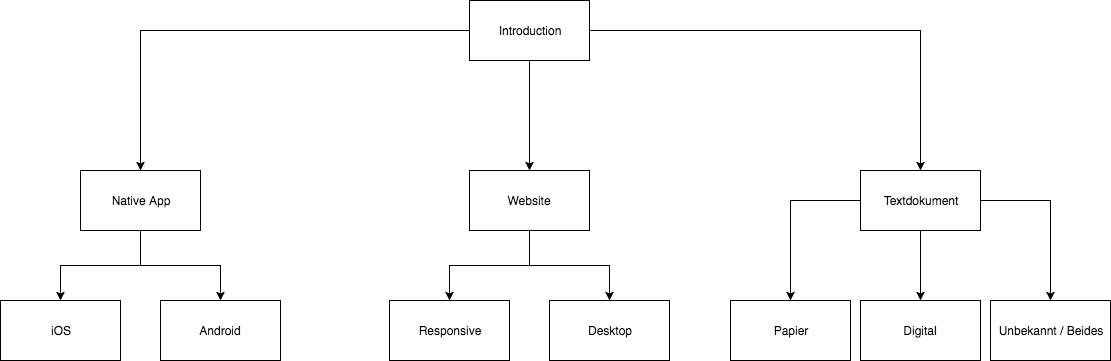
\includegraphics[width=1\textwidth]{images/ablauf_intro.png}
    \caption{Zielmedien der Nutzer und deren Unterkategorien}
    \label{fig:intro}
\end{figure}

Obwohl die Abgrenzung der Bereiche für die hier definierte Zielgruppe ausreichend ist, lassen sich bereits jetzt einige Stellen erkennen, die bei einer möglichen späteren Erweiterung der Zielgruppe überarbeitet werden müsste. Vorrangig betrifft das den Bereich \textit{Website}. Hier ist die vorhandene Unterteilung in \textit{Responnsive} und \textit{Desktop} für ein Echtwelt-Szenario unter Umständen zu allgemein gehalten.

Hier gilt es außerdem festzulegen, wie genau der Nutzer der Anwendung sein jeweiliges Zielmedium mitteilen soll. Ziel muss es dabei sein, die kognitive Arbeit\footnotemark{} diesen so gering wie möglich zu halten. Die in Abbildung \ref{fig:intro} gezeigte Struktur legt hier bereits eine Möglichkeit nahe, dem Nutzer immer nur eine Ebene des Baumes zur gleichen Zeit zu zeigen und so die Zahl der Auswahlmöglichkeiten so gering wie möglich zu halten.\\

\footnotetext{Als kognitive Arbeit werden Prozesse bezeichnet, die ein Nutzer durchführen muss, obwohl diese nicht sein eigentliches Anwendungsziel unterstützen. \cite[S. 410]{Cooper200903}}

Der Nutzer durchläuft einen Wizard\footnotemark{}, der maximal drei Auswahlmöglichkeiten zur gleichen Zeit darstellt. Zur weitern Unterstützung und zur einfacheren Identifizierbarkeit bestehen die Interface-Elemente für die verschiedenen Auswahlmöglichkeiten aus Icon und Text.
Zum Ende des Wizards wird dem Nutzer seine Auswahl noch einmal angezeigt, um so Fehler zu vermeiden, die unter Umständen zu einem späteren Zeitpunkt in der Anwendung den gesamten erarbeiteten Fortschritt nutzlos machen würde.

\footnotetext{"A \textbf{wizard} [...] is an enforced sequence of actions; [...]" \cite[S. 418]{Cooper200903}}

\section{Typographie}
Durch die Umsetzung des Bereiches Typographie als Proof of Concept innerhalb des Praxisprojektes war hier bereits viel grundlegende Konzeptarbeit verrichtet worden, auf der hier aufgebaut werden konnte. Die Grundlegende Interaktion wurde dabei beibehalten: Weiterhin sieht der Nutzer einen Text, der sich auf seine Eingaben hin verändert. Die Eingabe erfolgt weiterhin primär über Schieberegler, die über Tabs gruppiert sind. Die Platzierung dieser beiden Hauptelemente wurde aber verändert, sodass diese jetzt nebeneinander angeordnet sind, und nicht übereinander (vgl. Abbildung \ref{fig:vgl_poc_ba}). Das hat den Vorteil, dass der Nutzer weniger Scrollen muss und so die Möglichkeit hat, den Text und die Bedienelemente gleichzeitig zu sehen.\\
Eine weiter Verbesserung konnte im Bereich der Fehleranzeige vorgenommen werden: Hier wird über ein Icon in der Tab-Navigation deutlich gemacht, dass in einem bestimmten Bereich ein Fehler vorliegt.

\begin{figure}[h]
    \centering
    \includegraphics[width=1\textwidth]{images/vergleich_PoC_BA.png}
    \caption{Der Bereich Typographie, im Praxisprojekt und der Abschlussarbeit}
    \label{fig:vgl_poc_ba}
\end{figure}

Einen weiteren Ansatz stellt die direkte Interaktion mit Elementen dar. So bestünde beispielsweise die Möglichkeit, eine Überschrift anzuklicken und deren Attribute daraufhin direkt zu editieren. Hier wird, im Vergleich zur Interaktion mit Tab-Navigation und Schiebereglern, schneller deutlich, auf welches Element die gewählt Veränderung wirkt, jedoch bietet dieser Ansatz auch einige Nachteile. So können sich Elemente überschneiden (beispielsweise bei der Änderung der Breite des Textes und der Veränderung eines Textabsatzes), wodurch eine genaue Auswahl schwierig wird. Weiterhin ist diese Art der Interaktion nicht sehr verbreitet und würd eine Erklärung benötigen.\\
Um diese Probleme zu umgehen und allgemeine Einstellungen wie die Textfarbe oder die Schriftfamilie festzulegen, wäre also eine Vermischung der beiden Ansätze nötig. Weiterhin ergeben sich Probleme bei einer übersichtlichen Fehleranzeige: Es stellt sich als kompliziert dar, deutlich zu machen, zu welchem Attribut ein Fehler zugehörig ist.\\

Eine Konzeptuelle Neuerung stellt der Reset-Button dar. Dieser erlaubt ein einfaches zurücksetzen auf die Standardeinstellung und nimmt es dem Nutzer damit ab, im Zweifel 10 oder mehr Werte verändern zu müssen, um auf eine bestimmte Einstellung zurück zu kommen.\\
Im Bezug auf die Standardeinstellungen stellt sich die Frage, welche Einstellungen hier zu verwenden sind. Es wurde sich bewusst gegen eine fehlerfreie Standardeinstellung entschieden, da es dem Nutzer nicht möglich ist, in der Anwendung einen Schritt vorwärts zu gehen, wenn noch Warnungen angezeigt werden. So kann sicher gestellt werden, dass der Nutzer sich auf jeden Fall mit dem Bereich Typographie befasst.\\
Auf der anderen Seite sollten die Standardeinstellung nicht zu viele Fehler enthalten, um den Nutzer nicht zu demotivieren. Hier wurde nur ein einziger Fehlerhafter Wert gewählt, der im ersten Tab zu sehen und somit schnell zu beheben ist.\\

\section{Farben}
Während des Praxisprojektes wurde auch hier bereits ein grundlegendes Konzept aufgestellt. Die wichtigsten Punkte, in wenigen Sätzen zusammen gefasst, sind dabei:
Die Farbfindung geschieht in zwei Schritten, das finden der Grundfarbe und das Finden der Akzentfarbe. Farben sollen dabei auch nach Emotionen oder Adjektiven wählbar sein. Für die Betriebssysteme iOS und Android bestehen dabei gesonderte Regeln. \cite{PoplawskiPP}

Im ersten Schritt wurden die verschiedenen Darstellungen für die unterschiedlichen \textit{scopes} festgelegt.

\begin{itemize}
  \item \textbf{Finden einer Grundfarbe:} Hier wurde das Konzept aus dem Praxisprojekt übernommen. Für den jeweiligen \textit{scope} werden die jeweiligen Farben zu Auswahl gezeigt (wobei für die \textit{scopes} Website und Textdokument mit einem Colorpicker eine größere Auswahl an Farben besteht). Ist der \textit{scope} Android, so werden die Farben mit der Helligkeit 500 angezeigt und nach eine Auswahl durch den Nutzer die Abstufungen 300 und 500 automatisch hinzugefügt, um den Raum für Fehler so gering wie möglich zu halten.
  \item \textbf{Finden einer Akzentfarbe:} Für den \textit{scope} iOS entfällt dieser Schritt, für die beiden anderen Schritte wurde dem Nutzer die Möglichkeit gegeben, über Buttons die Art der Akzentfarbe zu wechseln (im Bereich Android über die Helligkeit, in anderen Bereichen in Form des gewählten Kontrastes).
  \item \textbf{Anzeigen des Farbschemas:} Wie bereits beim Einstieg in die Anwendung soll dem Nutzer am Ende das gesamte Farbschema angezeigt werden, bevor er zum nächsten Schritt in der Anwendung über geht. Dies ist vor allem Nötig, weil der Nutzer während der Erstellung immer nur Teile des gesamten Farbschemas sieht.
\end{itemize}

Die Zuordnung von Farben zu Adjektiven gestaltete sich dabei nicht ganz einfach. So machen viele Quellen, gerade im Bereich Marketing, zwar angaben über die Wirkung von Farben, aber genaue Farbabstufungen (zum Beispiel in Form von HEX- oder RGB-Werten) lassen sich nicht finden.
Ziel der Anwendung muss es aber sein, dem Nutzer einen Konkreten Wert zu geben, mit dem dieser Arbeiten kann. Da die Farbfindung über Adjektive hier vor allem den Zweck hat, das Finden einer Farbe für den Nutzer zu erleichtern, und nicht, die Farbwirkung des Artefakts des Nutzer möglichst auf eine Emotion zu bringen, wurde es hier als annehmbar angesehen, die genauen Farbabstufungen zufällig festzulegen. Konkret wurden aus [Artikel] 27 Adjektive extrahiert, zu denen Farbabstufungen gewählt wurden.

Wert wurde auch darauf gelegt, dem Nutzer die von ihm gewählte Farbe bereits währen der Auswahl in einem möglichen späteren Einsatz zu zeigen. Deswegen verfärbt sich ein großer Teil des Hintergrundes während dieses Schrittes entsprechend der Auswahl des Nutzers. Diese Hintergrundfärbung wird auch bei der Wahl der Akzentfarben beibehalten, wobei die Akzentfarben als keiner Flächen auf der Grundfarbe angezeigt werden, Auch hier soll ein direkter Einblick in die mögliche spätere Verwendung geschaffen werden. Abbildung ZXC zeigt diesen Ansatz im fertigen Produkt.

\section{Layouts \& Grid}

Auch für den Bereich “Layouts \& Grid” musste weitere, konkrete Konzeptionsarbeit geleitet werden.

Dieser Bereich unterscheidet sich zu den voran gegangenen vor allem dadurch, dass Nutzer mit Verschiedenen Entwicklungzielen hier deutlich verschiedene Interaktionen sehen. Der konkrete Ablauf kann dem Diagramm in Abbildung ZXC entnommen werden. Im folgenden sei der Ablauf anhand der einzelnen Knoten genauer erklärt.

Für Native Geräte ist hier nicht viel Interaktion vorgesehen. Bereits im Praxisprojekt wurde erkannt, dass die Mobilen Plattformen für sich ausreichend genaue Guidlelines in verschiedenen Formen bieten. Im Falle von Android ist in den Material Design Guidelines dabei für verschiedene Elemente sehr genau definiert, wie und mit welchem Abstand diese zu Platzieren sind, im Falle von iOS liefert der Storyboard-Editor von Xcode ausreichend genaue Richtlinien.
Aus diesen Gründen wird hier jeweils auf die Beiden Hilfestellungen hingewiesen und der Nutzer zum nächsten Schritt weiter geleitet.

Für Textdokumente wurde innerhalb des Praxisprojektes bereits eine recht genaue Interaktion konzipiert. Hier sollte es möglich sein, dass der Nutzer den Außenabstand des Dokumentes, ähnlich wie bei der Typographie, selbst verändert und die Anwendung ihm hier Hilfestellungen gibt. Weiterhin sollte die Möglichkeit gegeben werden, den Text in mehrere Spalten aufzuteilen. Diese Interaktion soll auch hier übernommen werden, Abbildung ZXD zeigt ein im Praxisprojekt erarbeitetes Wireframe und ein darauf basierendes, Innerhalt der Abschlussarbeit erstelltes Design.
Hier wurde lediglich die Anordnung verbessert, in dem das Dropdown in einer Reihe mit den anderen Bedienelementen angeordnet ist.
Konzeptionell stellt sich hier außerdem die Frage, ob eine Änderung der Reihenfolge für die verschiedenen Schritte, in der der Nutzer die Anwendung durchläuft für das Erstellen eines Textdokumentes nicht sinnvoll wäre. So könnte hier bereits die Textbreite definiert werden (durch die große des Dokumentes und die Anzahl der Spalten), so dass diese dann im Bereich Typographie fest gesetzt werden kann und der Text besser auf die jeweilige Breite angepasst werden kann.

Für den Bereich Web wurde im Praxisprojekt ein Vergleich verschiedener Grid-Systeme unternommen. Die Ergebnisse dieses Vergleiches sollen auch hier verwendet werden, in dem sie dem Nutzer zum Beispiel in der PDF als Mögliche Grid-Systeme nahe gelegt werden.
Die Anwendung an sich sollte hier aber auch noch einen Versuch unternehmen, den Nutzer an die generelle Arbeit mit Grid-Systemen heran zu führen. Dieser Schritt unterscheidet sich zu den anderen insoweit, dass dieser dem Nutzer kein Konkretes Ergebnis liefern, sondern ihm nur implizites Wissen vermitteln kann.
Der Gedanke hier ist es, den Nutzer mit verschiedenen Einstellungen für Grid-Systeme experimentieren und die Auswirkungen auf eine Seite beobachten zu lassen.

\section{Ergebnisse der Benutzung}
Auch wenn es eines der Hauptziele der Anwendung ist, dem Nutzer während seiner Nutzung interaktiv Wissen zu vermitteln, ist die Anwendung dennoch darauf ausgelegt, den Nutzer bei der Gestaltung eines konkreten Artefaktes zu unterstützen. Hier ist es für den Nutzer hilfreich, auf die von ihm erarbeiteten Ergebnisse auch nach der Verwendung des Tools noch Zugriff zu haben.

Dieser Bereich wurde im Rahmen des Praxisprojektes nicht konzipiert, ist aber für die Wahrnehmung der Anwendung als fertiges Produkt durchaus wichtig. Eine gute Darstellung der Ergebnisse des Nutzers definiert einen ausschlaggebenden Teil der Nutzungserfahrung, da ohne diesen Schritt das Gefühl aufkommen würde, dass während der Zeit der Nutzung kein Mehrwert erwirtschaftet wurde.
Im folgenden sollen also mögliche Darstellungen der Ergebnisse diskutiert und vorrangig die Frage beantwortet werden, welche Darstellungsweise den besten Kompromiss aus Umsetzbarkeit und Mehrwert für den Nutzer bietet.

Die einfachste Darstellung, die in jedem Falle gewählt werden sollte, ist eine transistente Darstellung am Ende eines Nutzung der Anwendung. Hier sollte dem Nutzer noch einmal aufgezeigt werden, welche Werte er innerhalb der Anwendung erarbeitet hat. Transistent ist diese Darstellung, weil diese zunächst nur im JavaScript-Programm im Browser des Nutzers gespeichert wird. Schließt dieser das Browserfenster, so wird auch das JavaScript-Programm beendet und die Ergebnisse gehen verloren.

Ein naheliegender Schritt ist also die Persistierung des Wissens für den Nutzer. Hierfür bieten sich verschiedene Möglichkeiten. \\
Denkbar wäre zum Beispiel das Speichern der Daten als Cookie im Browser des Nutzers. So könnten die Daten beim nächsten Besuch der Anwendung wieder angezeigt werden. Von Nachteil ist hier, dass die Kontrolle über die Speicherung der Daten nicht explizit beim Nutzer liegt: Löscht der Browser den Cookie (zum Beispiel, weil dessen \textit{Max-Age}\footnotemark{} Wert überschritten ist) sind die Daten ohne Eingriffsmöglichkeit des Nutzers verloren.
Eine andere möglichkeit Bietet das Entwicklen eine Backends, das eine entsprechende Datenhaltung verwalten kann. Hier könnten auch meherere Projekte eines Nutzer gespeichert werden. Allerdings liegt der Entwicklungsaufwand für ein solche Backend außerhalb des zeitlichen Rahmens der Abschlussarbeit. \\
Als Kompromiss zwischen Nutzerfreundlichkeit und Entwicklungsaufwand wurde sich für die Persistierung des Wissen in einer Datei im PDF-Format entschieden, die der Nutzer Herunterladen kann.

\footnotetext{Das \textit{Max-Age} Attribut kennzeichnet die maximale Dauer, die ein Cookie im Browser behalten wird. \cite{rfc6265}}

Weitere Verbesserungen der Nutzererfahrung können im Aufbau und Inhalt der Datei erreicht werden. Optimal wäre eine Aufbereitung der Daten, sodass der Nutzer diese möglichst ohne weitere Bearbeitung in seinen Workflow übernehmen kann. Obwohl das Zielmedium des Nutzers bekannt ist, können daraus keine zweifelsfreien Rückschlüsse auf die benötigte Struktur und Form der Daten gezogen werden. \\
So kann beispielsweise bekannt sein, dass der Nutzer eine Webanwendung entwickelt und das Styling für seine Texte in CSS vornimmt. Trotzdem kann der Nutzer zum Beispiel verschieden Preprozessoren wie SCSS, SASS oder LESS verwenden, die alle eine unterschiedliche Syntax verwenden.
Oder es kann bekannt sein, dass der Nutzer an einer Textseite arbeitet, jedoch nicht, welches Textsatzprogramm er verwendet\footnotemark{}.\\
\footnotetext{Ein weiteres Problem stellt die Aufbereitung der Daten für einen Import in ein Textsatzprogramm dar.}
Es is dabei durchaus Möglichen, die benötigten Informationen vom Nutzer zu erhalten und die Daten in Einzelfällen entsprechend aufzubereiten, jedoch liegen auch diese Anforderungen außerhalb des Zeitlichen Rahmens dieser Abschlussarbeit.

\chapter{Technischen Grundlagen}
\thispagestyle{fancy}
Das nachfolgende Kapitel soll die technischen Grundlagen erläutern, die für die Umsetzung der Anwendung von Bedeutung sind. Im Folgenden sollen verschiedene Möglichkeiten der Umsetzung diskutiert und der Prozess für die Wahl der verwendeten Technologien und Frameworks erläutert werden.\\
Weiterhin sollen im zweiten Teil dieses Kapitels die nötigen Grundlagen für ein Verständnis des Aufbaus der Anwendung und ihres Quellcodes geschaffen werden.

\section{Diskussion verfügbarer Technologien}
Durch die in Kapitel \ref{chap:concept} definierten Konzepte können bereits einige Anforderungen an die Anwendung gefunden werden, die für die Umsetzung von Bedeutung sind.
Die Anwendung:

\begin{itemize}
  \item weist einen hohen Grad der Interaktivität auf
  \item benötigt kein Backend
  \item soll eine Webanwendung sein
\end{itemize}

Die Anwendung entspricht somit einer \textit{Rich Internet Application} wie sie George Lawton definiert:

\begin{quote}
  RIAs feature responsive user interfaces and interactive capabilities. This makes Internet-based programs easier to use and more functional, and also overcomes problems with traditional Web applications such as slow performance and limited interactivity \cite{lawton2008new}
\end{quote}

\subsection{Rich Internet Applications}
Die Idee, Webseiten dynamischer und interaktiver zu gestalten geht dabei fast so weit zurück wie die Idee des Internet selbst.

\begin{quote}
  Very early on, software engineers realized that the client-server architecture of the Web provided a powerful platform in which the browser could be a universal user interface to applications that may run locally or remotely on a server \cite{Jazayeri:2007:TWA:1253532.1254719}
\end{quote}

Um diese Interaktivität und Dynamik umzusetzen, wurden zunächst Plattformen mit eigenen Laufzeitumgebungen genutzt. Lawton nennt hier beispielsweise Microsoft Silverlight, Adobe Flash oder JavaFX  \cite{lawton2008new}.
Die Verwendung von eigenen Laufzeitumgebungen dieser Plattformen  bedeutete für den Nutzer jedoch,  dass dieser bestimmte Programme auf seinem Rechner, oder Plug-ins in seinem Browser installieren musste, um Zugriff auf die so mögliche Interaktivität zu erhalten. Auf einen der größten Vorteile der Entwicklung von Webanwendungen, das Ausführen der Anwendung ohne vorherige Installation, musste somit verzichtet werden.

Durch das Verabschieden von neuen Web-Standards wie HTML5 oder ECMAScript 6 können viele Funktionen der oben genannten Plattformen nativ in einem Browser abgebildet werden. So empfiehlt Adobe beispielsweise, Flash nicht für Funktionen zu nutzen, die auch mit Hilfe von HTML5 abgebildet werden können\footnotemark{}.\\
Für die Realisierung dieser Interaktivität im Browser wird vor allem JavaScript verwendet.

\footnotetext{siehe dazu \url{https://blogs.adobe.com/conversations/2015/11/flash-html5-and-open-web-standards.html}, zuletzt abgerufen am 11.08.2017}

\subsection{Single Page Applications}
Das Prinzip der \textit{Single Page Applications (SPAs)} lässt sich bereits an der Wortbedeutung gut erkennen: Es handelt sich um Anwendungen, die auf einer einzigen HTML-Seite ausgeliefert werden.
Mikowski und Powell definieren SPAs als

\begin{quote}
  […] an application delivered to the browser that doesn’t reload the page during use. Like all applications, it’s intended to help the user complete a task, such as “write a document” or “administer a web server.” We can think of an SPA as a fat client that’s loaded from a web server. \cite{MikowskiPowell201309}
\end{quote}

\textit{Single Page Applications (SPAs)} können somit als Untereinheit der \textit{Rich Internet Applications} bezeichnet werden.\\
Eine der ältesten Möglichkeiten, eine \textit{Single Page Application} zu realisieren stellt AJAX dar. AJAX erlaubt das Nachladen von Inhalten vom Server, ohne das erneute Laden der im Client geöffneten Seite zu erzwingen \cite{paulson2005building}.\\
Da eine Anforderung an die zu entwickelnde Anwendung aber die Absenz eines Backends ist, kann AJAX als Möglichkeit zur Umsetzung ausgeschlossen werden.

Aufgrund der Möglichkeiten, die mit den bereits erwähnten, neuen Web-Standards einhergehen, entstanden in den letzten Jahren jedoch viele JavaScript-Frameworks, die sich auf die Entwicklung von \textit{Single Page Applications (SPAs)} spezialisieren.


\subsubsection{JavaScript Single Page Application Frameworks}

Aus der Menge der verfügbaren JavaScript-Frameworks, die sich für die Umsetzung einer \textit{SPA} eignen, wurden hier drei für eine Untersuchung auf die Tauglichkeit für die Umsetzung der konzipierten Anwendung hin untersucht.
Die Auswahl der Frameworks erfolgte dabei nach Verbreitung und tatsächlicher Verwendung.\\
Da sich die genaue Messung der Verbreitung einer Software schwierig gestaltet, wurde als Indikator für die Beliebtheit und Verbreitung die Zahl der \textit{stars}\footnotemark{}, die den verschiedenen Frameworks auf der Plattform GitHub  zugeordnet sind, verwendet.

\footnotetext{Ein \textit{star} sagt aus, dass eine Person Interesse an dieser Software zeigt.}

Im Folgenden werden die Frameworks Vue.js, Angular.js und React.js verglichen.

\textbf{Vue.js} \cite{vue} wurde im Dezember 2013 veröffentlicht.
Vue beschreibt sich selbst in der Einführung der Dokumentation wie folgt:

\begin{quote}
  Vue […] is a progressive framework for building user interfaces. Unlike other monolithic frameworks, Vue is designed from the ground up to be incrementally adoptable. The core library is focused on the view layer only, and is very easy to pick up and integrate with other libraries or existing projects. \cite{VueIntro}
\end{quote}

Vue.js ist dabei, wie die anderen hier behandelten Frameworks, Komponentenbasiert. Um das User Interface effektiv zu aktualisieren, verwendet es einen \textit{Virtual DOM}. Dieser ist eine Abstraktion des DOMs, wie ihn beispielsweise das W3C spezifiziert:

\begin{quote}
  The Document Object Model (DOM) is a programming API for HTML and XML documents. It defines the logical structure of documents and the way a document is accessed and manipulated.  \cite{w3cDOM}
\end{quote}

Das \textit{Virtual DOM} wird von Frameworks wie Vue.js dafür verwendet, Änderungen am DOM performanter durchführen zu können. Die genaue Funktionsweise sei im Rahmen dieser Arbeit nicht erläutert, jedoch beschreibt die Vue.js Dokumentation die abstrakten Vorgänge wie folgt:

\begin{quote}
  Under the hood, Vue compiles the templates into Virtual DOM render functions. Combined with the reactivity system, Vue is able to intelligently figure out the minimal amount of components to re-render and apply the minimal amount of DOM manipulations when the app state changes. \cite{VueTemplate}
\end{quote}

Für das Darstellen von Inhalten verwendet Vue.js eine Templating-Engine, Erweiterungen, wie Routing oder Verwaltung des Zustandes der Anwendung, müssen über externe Bibliotheken eingefügt werden.

Das von Google entwickelte Framework \textbf{Angular.js} \cite{angular} ist das älteste der hier behandelten Frameworks, die erste Version wurde im Oktober 2010 veröffentlicht.\\
Insgesamt ist Angular deutlich komplexer als Vue.js und React.js. Viele Erweiterungen, wie zum Beispiel das Routing, die in Vue.js und React.js durch externe Bibliotheken implementiert werden müssen, sind beispielsweise in Angular.js bereits enthalten.
Auch weisen Angular-Anwendungen eine deutlich komplexere Architektur auf, die unter anderem aus Teilen wie Modulen, Komponenten und Templates besteht. Hier wird für die Darstellung von Inhalten ebenfalls eine Templating-Engine verwendet.

\textbf{React.js} \cite{react} wurde im Juli 2013 von Facebook veröffentlicht.\\
Wie Vue.js implementiert auch React.js ein Virtual DOM, um Änderungen in der Benutzeroberfläche performanter abbilden zu können.
Anders als Vue.js und Angluar.js verwendet React jedoch keine Templating-Engine, React-Anwendungen sind daher als komplett in JavaScript-Funktionen geschrieben, die zur Laufzeit in HTML umgewandelt werden.
Ähnlich wie Vue.js ist auch React.js in seiner Funktionalität sehr auf die wesentlichen Funktionen reduziert, Erweiterungen wie Routing oder die Verwaltung des Zustandes der Anwendung müssen auch hier über externe Bibliotheken eingebunden werden.

Aus dem Vergleich wird zunächst deutlich, dass alle Frameworks ähnliche Ziele verfolgen und somit auch jedes der betrachteten Frameworks für die Umsetzung der hier vorliegenden Anwendung grundsätzlich geeignet sind.
Angular.js wurde ausgeschlossen, da die relativ komplexe Grundstruktur für eine eher kleinere Anwendung, wie sie hier entwickelt werden soll, als unpassend erachtet wurde.
Die abschließende Entscheidung fiel auf das Framework React.js, aus dem pragmatischen Grund, dass bereits im Vorfeld dieser Arbeit ein Proof of Concept entstand, der ebenfalls auf dem Framework React.js aufbaut. Hiervon wurde sich ein simpleres Übertragen bestimmter Teile aus dem Proof of Concept versprochen.


\section{Einstieg in React.js}
Das Framework React.js definiert einige spezielle Konzepte und Vorgänge, auf die im Folgenden eingegangen werden soll. Der Umfang soll dabei so gering wie möglich bleiben, aber trotzdem ein Verständnis der später in dieser Arbeit gezeigten Codebeispiele und des Quellcodes auf der beiliegenden CD ermöglichen.

\subsection{Komponenten}
Die komponentenbasierte Entwicklung ist einer der Hauptbestandteile der Architektur einer React-Anwendung \cite[S. 28]{Gackenheimer201509}. \\
Dieser Abschnitt beschäftigt sich mit dem Aufbau, der Verwendung, den verschiedenen Formen und den Besonderheiten von Komponenten in React.\\
Bevor auf die Besonderheiten von Komponenten in React.js eingegangen wird, soll im Folgenden zunächst ein Überblick über das Konzept der Komponente an sich und im Kontext der Software-Entwicklung gegeben werden.

\subsubsection{Was ist eine Komponente?}
\label{chap:component}
Als erster Schritt zu Beantwortung der Frage, was eine Komponente ist, bietet sich die Betrachtung der Wortbedeutung an. Der Duden definiert eine Komponente als "Bestandteil eines Ganzen" \cite{Dudenredaktion2006}. Diese Definition gibt bereits erste Hinweise auf die Eigenschaften einer Komponente in der Software-Entwicklung.\\
Weitere Eigenschaften definiert Clemens Szyperski:

\begin{quote}
  One thing can be stated with certainty: components are for composition. […] Composition enables prefabricated “things” to be reused by rearranging them in ever-new composites. \cite{Szyperski200211}
\end{quote}

Und De Alfredo und Henzinger schreiben über Komponenten:

\begin{quote}
  It does not constrain the environment but describes the behavior of the component in an arbitrary environment: “for all inputs x and y, if y $\neq$ 0, then the output is z = x/y“ \cite{de2001interface}
\end{quote}

Für den Rahmen dieser Arbeit können daraus für Komponenten also folgende Eigenschaften gefolgert werden:\\
Eine Komponente ist nur ein einzelner Teil der ganzen Anwendung. Dieser Teil sollte (nach Möglichkeit) auch an anderen Stellen in der Anwendung wiederverwendbar sein und sollte weiterhin keine Abhängigkeit von seiner Umwelt besitzen.

\subsubsection{Komponenten in React.js}
Die React.js-Dokumentation selbst enthält eine weitere Definition einer Komponente:

\begin{quote}
  Conceptually, components are like JavaScript functions. They accept arbitrary inputs (called "props") and return React elements describing what should appear on the screen. \cite{ReactProps}
\end{quote}

Jede Komponente in React.js ist eine Subklasse der Basisklasse \verb|React.Component| und besitzt einen Lebenszyklus, den sogenannten \textit{Component Lifecycle}. Dieser besteht aus drei Zuständen \cite{ReactCom}:

\begin{enumerate}
  \item Mounting
  \item Updating
  \item Unmounting
\end{enumerate}

Für jeden dieser Zustände können verschiedene Funktionen aus der Basisklasse \verb|React.Component| überschrieben werden, um diese in der Komponente zu verwenden.

\textit{Mounting} und \textit{Unmounting} beschreiben den Anfang beziehungsweise das Ende des Lebenszyklus und Funktionen, die diesen Zuständen zugehörig sind, werden demnach nur einmal aufgerufen.
Funktionen, die  dem Zustand \textit{Updating} zugehörig sind, können beliebig oft aufgerufen werden. Dieser Aufruf geschieht jedes Mal, wenn ein Update der Komponente initiiert wird. Von besonderer Bedeutung ist hier die Funktion \verb|render()|, in der definiert wird, welchen Inhalt die Komponente ausgeben soll.

Für das Arbeiten mit Komponenten in React ist weiterhin das Konzept der \textit{props} und des \textit{state} relevant \cite{ReactProps}.\\
Dabei bezeichnen \textit{props} JavaScript-Objekte, die von einer Elternkomponente zur Kindkomponente übergeben werden können. Besonders interessant ist die Möglichkeit, Referenzen auf Funktionen übergeben zu können. Somit kann in einer Elternkomponente auf die Interaktion mit einer Kindkomponente reagiert werden.\\
Der \textit{state} bezeichnet im weitesten Sinne den Zustand einer Komponente. Dieser Zustand ist ein Attribut einer Komponente, in dem Werte gespeichert werden, die für die Anzeige des Zustandes der Komponente relevant sind (zum Beispiel, welche Kindkomponente als aktiv dargestellt werden soll).\\

Hier zeigt sich außerdem der Grundgedanke der Interaktivität in React.js: Werden \textit{props} oder \textit{state} aktualisiert, werden die Funktionen des \textit{Updating}-Zustandes im Lebenszyklus dieser Komponente aufgerufen. Somit kann die Ausgabe der Komponente auf die neuen Werte angepasst werden.

\subsubsection{Zustandslose Komponenten}
\label{chap:stateless}
Nicht jede Komponente in React.js muss einen Zustand verwalten, viele Komponenten innerhalb einer Anwendung dienen nur der Darstellung von Inhalten, die ihnen von ihren Elternkomponenten übergeben werden. Vor den in Kapitel \ref{chap:component} definierten Anforderungen an eine Komponente ist es Sinnvoll, viele in sich abgeschlossene und in ihren Funktionen limitierte Komponenten zu implementieren, die dann von einigen wenigen Komponenten kontrolliert werden.\\
Da zustandslose Komponenten keine der im vorhergehenden Kapitel erwähnten Methoden des Lebenszyklus implementieren, wurde mit dem Release von React 0.14\footnotemark{} eine simplifizierte Schreibweise für diese Komponenten eingeführt (Listing \ref{lst:stateless} zeigt diese). Hier wird zum einen das unnötige Schreiben von Code vermeiden, zum anderen kann während der Entwicklung auf den ersten Blick festgestellt werden, ob eine Komponente einen Zustand verwaltet oder nicht.

\footnotetext{Siehe dazu \url{https://facebook.github.io/react/blog/2015/09/10/react-v0.14-rc1.html}, zuletzt abgerufen am 11.08.2017}

\begin{lstlisting}[caption={Simplifizierte Schreibweise für Komponenten ohne \textit{state}}, label=lst:stateless]
  const Button = (props) => {
  	return (
  		<button onClick={props.onClick}>Click me!</button>
  	)
  }

  export default Button
\end{lstlisting}

Ein Beispiel für die Verwendung von Komponenten mit und ohne \textit{state} innerhalb der hier geschriebenen Anwendung findet sich in Kapitel \ref{chap:state_component}.

\subsection{JSX}
\label{chap:jsx}
JSX ist eine (eigens von Facebook für die Verwendung mit React entwickelte) Syntax-Erweiterung für ECMAScript, die es Erlaubt, React-Komponenten innerhalb der \verb|render()|-Methode ähnlich wie HTML-Tags zu deklarieren.

JSX ist dabei lediglich eine syntaktische Verschönerung der Funktion \verb|React.createElement(component, props, ...children)| \cite{ReactJSX}, die für die tatsächliche Definition von Komponenten verwendet wird.
Obwohl die JSX-Syntax der HTML-Syntax ähnlich sieht, gibt es hier einige Besonderheiten, die beachtet werden müssen.
Zum einen werden die Deklarationen von React-Komponenten und regulären HTML-Tags durch unterschiedliche Schreibweisen getrennt (React-Komponenten werden groß geschrieben) zum anderen können hier keine Schlüsselwörter verwendet werden, die durch die ECMAScript-Spezifikation geschützt sind\footnotemark{}. Dies betrifft in erste Linie das \verb|class|-Attribut, das in HTML für das Vergeben von Klassen verwendet wird. Für die Vergabe von CSS-Klassen muss in JSX auf \verb|className| zurück gegriffen werden.

\footnotetext{\url{https://developer.mozilla.org/en-US/docs/Web/JavaScript/Reference/Lexical_grammar}}

\section{Einstieg in Redux}
Mit zunehmender Komplexität einer React-Anwendung kann das Verwalten von Zuständen unübersichtlich werden. Diese Gefahr besteht vor allem dann, wenn Zustände über verschiedene Bestandteile der Anwendung hinweg bekannt sein müssen.

Um den Zustand einer Anwendung an einem zentralen Ort verwalten und diesen strukturiert verändern zu können, kann die Bibliothek Redux\footnotemark{} verwendet werden. In ihrer Dokumentation wird das Ziel der Bibliothek Ziel wie folgt:

\footnotetext{\url{http://redux.js.org/}, zuletzt abgerufen am 11.08.2017}

\begin{quote}
  \textbf{Redux attempts to make state mutations predictable} by imposing certain restrictions on how and when updates can happen. \cite{ReduxMotivation}
\end{quote}

Für ein Grundverständnis der Funktionsweise der Bibliothek sind drei Konzepte von Bedeutung:

\begin{itemize}
  \item \textit{Store}
  \item \textit{Actions}
  \item \textit{Reducer}
\end{itemize}

Der \textit{Store} ist ein JavaScript-Objekt, in dem der Zustand der Anwendung gespeichert ist. \textit{Actions} beschreiben, welche Veränderungen am \textit{Store} vorgenommen werden sollen. Auch diese sind einfache JavaScript-Objekte. \textit{Reducer} definieren, auf welche Weise der Zustand der Anwendung bei Aufruf einer \textit{Action} verändert werden soll. \cite{ReduxCore}

Die Implementierung von Redux in der hier zu entwickelnden Anwendung wird in Kapitel \ref{chap:redux} beschrieben.

\chapter{Umsetzung der Anwendung}
\thispagestyle{fancy}
Im Folgenden soll die Umsetzung der Anwendung thematisiert werden. Umsetzung meint hier sowohl die Programmierung der Anwendung und alle Bereiche, die mit dieser zusammen hängen, als auch die visuelle Gestaltung. Dieses Kapitel geht auf Konzepte ein, die während der Gestaltung der Anwendung eine zentrale Rolle spielten und schildert das generelle Vorgehen. Es werden einige strukturelle Entscheidungen erläutert, die während der Umsetzung von Relevanz waren und einige konkrete Codebeispiele gezeigt, die als besonders interessant erachtet wurden.

\section{Gestaltung}
Bereits in Kapitel \ref{sec:relevance} wird deutlich, welche zentrale Rolle die Gestaltung in jedwedem Projekt einnimmt. Auch das hier bearbeitete Projekt ist davon nicht ausgenommen. Um eine gute Benutzbarkeit des Tools zu gewährleisten, ist eine solide Gestaltung unabdingbar.\\
Steve Krug schreibt über die Gestaltung von Webseiten:

\begin{quote}
  Die Seiten offensichtlich zu gestalten, ist wie eine gute Beleuchtung in einem Geschäft: Alles erscheint einfach besser. Die Nutzung einer Website, die uns nicht zum Nachdenken über Unwichtiges zwingt, fühlt sich mühelos an, wogegen das Kopfzerbrechen über Dinge, die uns nichts bedeuten, Energie und Enthusiasmus raubt — und Zeit. \cite[S. 19]{Krug201410}
\end{quote}

Insgesamt ist \textit{25knots} eine sehr interaktive Anwendung, in der Informationen eher Grafisch und durch Interaktionen des Benutzers übertragen werden, als beispielsweise durch Texte.
Daher wurde bei der Gestaltung großer Wert darauf gelegt, klar zu kommunizieren, welche Bereiche interaktiv sind und welche Auswirkungen eine Interaktion mit diesen Bereichen hat.\\
Um diese Abgrenzung zu gewährleisten, wurde ein schlichtes Farbschema verwendet, in dem nur zwei Farben, Blau und Rot, verwendet wurden, die zur Anzeige von Interaktivität dienen.
Die beiden Farben haben dabei festgelegte Rollen: Blau zeigt Interaktivität innerhalb eines Schrittes der Anwendung an, Rot zeigt zwischen verschiedenen Schritten übergreifende Aktivitäten an. Abbildung \ref{fig:entrance} zeigt die Ausführung dieser Idee am Beispiel des Einstiegs in die Anwendung. Die blauen Elemente erlauben eine Auswahl innerhalb des Einstiegs (nächster Zwischenschritt, Auswahl eines Entwicklungsziels), der rote Button am unteren Rand erlaubt das Wechseln zum nächsten Abschnitt in der Anwendung.

\begin{figure}[h]
    \centering
    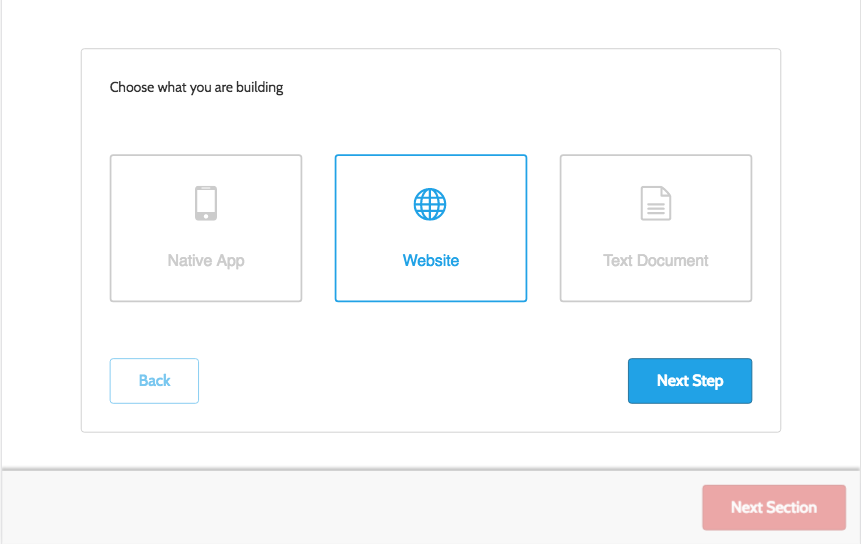
\includegraphics[width=1\textwidth]{images/25knots_entrance.png}
    \caption{Farben verschiedener interaktiver Elemente}
    \label{fig:entrance}
\end{figure}

Weiterhin gilt es zu beachten, dass der Nutzer die Anwendung verwendet, um eine Gestaltung für sein Projekt zu erstellen. Der Fokus der Anwendung sollte daher darauf liegen, dem Nutzer die von ihm erarbeitete Gestaltung zu zeigen. Die Anwendung selbst sollte sich nur in bestimmten Fällen (beispielsweise beim Auftreten eines Fehlers oder wenn eine Interaktion notwendig ist) in den Vordergrund stellen. Daher wurde darauf geachtet, die Anwendung so simpel wie möglich zu gestalten und auf unnötige gestalterische Experimente zu verzichten. Der größte Teil der Anwendung ist in Weiß- und Grautönen gehalten, um die Gestaltung des Nutzers und dessen Entscheidungen besser in den Vordergrund stellen zu können.

Dieses Vorgehen lässt sich anhand von zwei Beispielen gut verdeutlichen.\\
Als Erstes seien hier die Fehlermeldungen im Bereich Typographie genannt (siehe Abbildung \ref{fig:warning}). Diese sind in einem auffälligen Gelb hinterlegt, das nur für diesen bestimmten Anwendungsfall (das Hervorheben von Fehlern) verwendet wird und dem Nutzer dadurch schnell auffällt.\\
Auch zeigt die Auswahl von Farben für die Zielmedien Android und iOS (siehe Abbildung \ref{fig:accent}), wie interaktive Elemente verwendet wurden, um dem Nutzer bereits einen Eindruck der von ihm erstellten Gestaltung zu geben. Die Buttons zeigen lediglich die Farbe selbst, mit deren Auswahl sie verbunden sind. Die Gestaltung der Anwendung tritt hier komplett in den Hintergrund.

\begin{figure}[h]
    \centering
    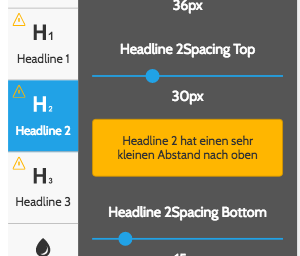
\includegraphics[width=0.5\textwidth]{images/25knots_Warning.png}
    \caption{Fehlermeldungen im Bereich Typographie}
    \label{fig:warning}
\end{figure}

\begin{figure}[h]
    \centering
    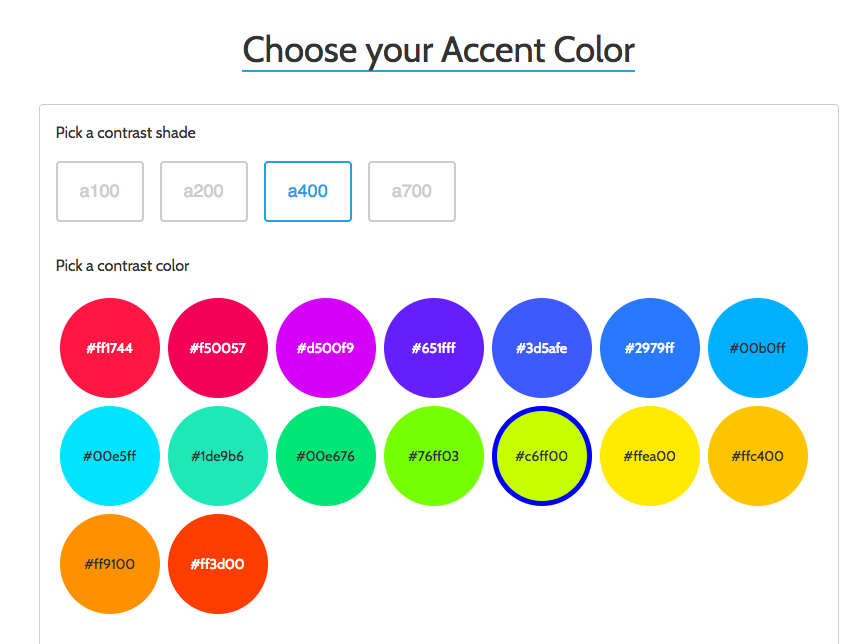
\includegraphics[width=1\textwidth]{images/25knots_color_button.png}
    \caption{Buttons zum Auswählen einer Akzentfarbe}
    \label{fig:accent}
\end{figure}


\subsection{Vorgehen}
Das Vorgehen während der Gestaltung lässt sich als agil bezeichnen. Diese Agilität drückt sich auf verschiedene Weise aus.\\
Der Entwicklungsprozess (gemeint ist hier die tatsächliche Programmierung) und der Gestaltungsprozess (das Erstellen von Mock-Ups in einem entsprechenden Grafikprogramm) waren nicht strikt voneinander getrennt, sondern überschnitten sich. Diese Überschneidung zeigt sich sowohl in einer langfristigen, als auch in einer kurzfristigen Betrachtung.\\
So gab es nicht einen Gestaltungsprozess, nach dessen Fertigstellung die Entwicklung startete, sondern vielmehr einen Gestaltungsprozess pro Schritt der Anwendung, der umgesetzt wurde.\\
Auch innerhalb eines Schrittes war das Vorgehen nicht linear, häufig wurden während der Entwicklung Aspekte in der Gestaltung verändert. Die Gründe hierfür liegen vor allem in den verbesserten Möglichkeiten zum Testen und Validieren von Interaktionen und Konzepten in einer prototypischen Realisierung im Vergleich zu statischen Mock-Ups.
Durch die in Kapitel \ref{chap:spacing} und \ref{chap:styleguide} erläuterten Aspekte konnten außerdem problemlos kleinere Änderungen in der Gestaltung während der Entwicklung vorgenommen werden, ohne dass dabei ein vorheriges Anpassen der Mock-Ups nötig war.\\
Alle im Rahmen der Arbeit erstellten MockUps finden sich auf der beiliegenden CD.

\subsection{Abstände}
\label{chap:spacing}
Um den Gedanken von innerhalb der Anwendung wiederverwendbaren Komponenten zu unterstützen liegt der Gedanke nahe, auch Abstände innerhalb der Gestaltung (und später auch in der Umsetzung) wiederverwendbar zu entwerfen. Die Grundlage für diesen Gedanken lieferte ein Artikel von Nathan Curtis \cite{CurtisSpace16}. Der Artikel enthält zwei Grundgedanken:

\begin{enumerate}
  \item Die Größen von Abständen sollten festgelegt und ihre Anzahl übersichtlich sein.
  \item Es gibt verschiedene Arten von Abständen, die die verschiedenen Größen auf unterschiedliche Weise einsetzen und kombinieren.
\end{enumerate}

Diese Gedanken wurden in der Gestaltung und Umsetzung des Projektes übernommen. Zunächst wurden die verschiedenen Abstände, aufbauend auf der von Curtis empfohlenen Basisgröße von \texttt{16px}, definiert. Aufbauend auf der Basisgröße wurden anschließend Abstufungen in beide Richtungen
erstellt, die nach Kleidergrößen, von XS bis XXL, benannt wurden.
Diese Abstufungen wurden in einer eigenen Datei als JavaScript-Objekt deklariert, so dass über die gesamte Anwendung hinweg diese festgelegten Größen verwendet werden können.

\begin{figure}[h]
    \centering
    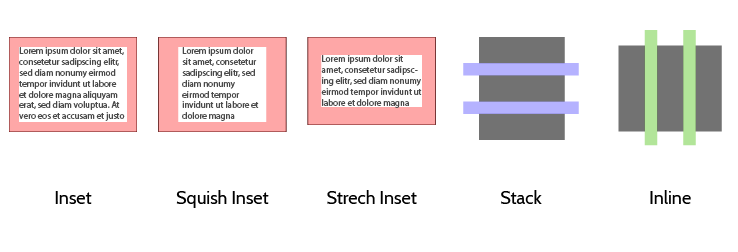
\includegraphics[width=1\textwidth]{images/spacing_types.png}
    \caption{Die 5 implementierten Arten von Spacing nach \cite{CurtisSpace16}}
    \label{fig:spacing}
\end{figure}


Curtis definiert 6 verschieden Arten von Abständen, von denen 5 innerhalb der Anwendung als eigenständige Komponenten definiert wurden (siehe Abbildung \ref{fig:spacing}).\\
Die Komponenten nehmen die Größe des Abstandes als \texttt{prop} in einer der definierten Kleidergrößen entgegen und erzeugen ein \texttt{div} Element, das die Abstände als \texttt{padding} oder \texttt{margin} anwendet.
Die Pixelwerte für die jeweilige Abstandsgröße erhält die Komponente dabei durch den Aufruf des für die Abstandsgrößen zuständigen JavaScript-Objekts (zum Beispiel \texttt{spacing.l}). Alle diese Komponenten geben außerdem die ihnen übergebenen Kinder aus, sodass eine Verwendung der \texttt{SpacingInset} Komponente wie in Listing \ref{lst:spacingInset} möglich wird.

\begin{lstlisting}[caption=Beispielhafte Verwendung einer Komponente für Abstände, label=lst:spacingInset]
  <SpacingInset size='l' >
    <h1> A Headline </h1>
    <p> Some Text </p>
  </SpacingInset>
\end{lstlisting}

Hier stellt sich die Frage, inwiefern es Sinn ergibt, Komponenten zu definieren, die eine ausschließlich visuelle Funktion haben.
So könnte deren Funktion auch innerhalb der CSS-Regeln von anderen Komponenten definiert und so ein übersichtlicheres Markup geschaffen werden.\\
Während der Arbeit stellte sich heraus, dass die Definition der Abstände als eigene Komponenten ein sehr einfaches Entwickeln von Interfaces ermöglichte. Durch die eingegrenzten Möglichkeiten ist auch während der Entwicklung ein Testen von anderen Abständen sehr einfach möglich.\\
Weiterhin ist der Raum für Inkonsistenzen begrenzt, da die Abstände nur in den vorgegebenen Größen angegeben werden können. Dies wurde, besonders mit Blick auf die spätere Weiterentwicklung und Veröffentlichung, als ausreichend großer Vorteil angesehen, um eine Definition als eigenständige Komponente zu rechtfertigen.

\subsection{Styleguide}
\label{chap:styleguide}
Da zu einem späteren Zeitpunkt unter Umständen verschiedene Personen an der Weiterentwicklung der Anwendung beteiligt sein werden, macht das Festhalten der bisher gestalteten Elemente und der Grundlagen der Gestaltung durchaus Sinn.
Während der Gestaltung wurde nur ein minimalistischer Styleguide mit Informationen über Farben, Schriftgrößen und Abstände geführt, der für die Gestaltung dieser ersten Version mit nur einer beteiligten Person ausreichend war.

Vor dem Hintergrund einer späteren Weiterentwicklung ist ein zentraler Ort, der einen Überblick über die bereits erstellten Komponenten gibt, von großem Vorteil.
Hierfür wurde die Bibliothek Storybook\footnotemark{} verwendet. Die Bibliothek wird lokal im Browser ausgeführt und ermöglicht es, verschiedene Komponenten aus der Anwendung gekapselt darzustellen. Hierbei ist zusätzlicher Code notwendig, die Komponenten können direkt aus dem Anwendungscode übernommen werden.
Die Bibliothek bietet dadurch außerdem den Vorteil, dass Komponenten zunächst alleinstehend entwickelt werden können, ohne dass diese in die eigentliche Anwendung eingebunden werden müssen.

\footnotetext{\url{https://github.com/storybooks/storybook}}

\section{Redux}
\label{chap:redux}

Im Laufe der Verwendung müssen bestimmte Informationen über die gesamte Anwendung hinweg für bestimmte Komponenten abrufbar sein. Dies betrifft vor allem, aber nicht ausschließlich, die vom Nutzer zu Beginn der Interaktion mit der Anwendung definierten Entwicklungsziele, die in jedem Bereich der Anwendung für die korrekte und auf das jeweilige Ziel angepasste Darstellung der  Inhalte überprüft werden.\\
Ein weiteres Beispiel stellt die Zusammenfassung am Ende der Interaktion mit der Anwendung dar, für die ein Zugriff auf alle vom Nutzer definierten Werte nötig ist. Der Redux-Store für die Anwendung umfasst daher Werte aus den Bereichen \textit{Intro}, \textit{Typographie} und \textit{Farben}.\\

Um die Arbeit mit dem Store zu simplifizieren und eine übermäßige Ver­schach­te­lung des Store-Objekts zu vermeiden, wurde für jeden der oben genannten Bereiche ein eigener \textit{Reducer} geschrieben, der ausschließlich für die Bearbeitung der diesem Bereich zugehörigen Werte verantwortlich ist.\\
In der Datei \texttt{ApplicationState.js} werden diese mit Hilfe der Funktion \texttt{combineReducers}, die von Redux zur Verfügung gestellt wird, dann zu einem Objekt zusammengefügt (siehe Listing \ref{lst:combine_reducer}).

\begin{lstlisting}[caption={Zusammenfügen der dedizierten Reducer zu einem Objekt}, label=lst:combine_reducer]
  const ApplicationState = combineReducers({
    setup: setup,
    typography: typography,
    colors: colors
})
\end{lstlisting}

\subsection{Beispielhaftes Verändern des Redux-Store}
Das Verändern des Redux-Store soll im Folgenden an einem konkreten Beispiel verdeutlicht werden. Das Szenario, das der Nutzer durchläuft, ist dabei das Auswählen einer Grundfarbe. In diesem Szenario hat der Nutzer bereits eine Wahl über seine Grundfarbe getroffen und möchte seine Auswahl nun durch den Klick auf den \textit{Next Step} Button bestätigen und zum nächsten Schritt übergehen (vergleiche hierzu Abbildung \ref{fig:colors_bg} auf Seite \pageref{fig:colors_bg}).\\
Für die Anwendung bedeutet diese Interaktion: Die aktuell gewählte Grundfarbe muss in den Redux-Store geschrieben\footnotemark{} und der nächste Schritt für die Farbfindung angezeigt werden. Dieses Beispiel soll sich dabei auf das Schreiben der Grundfarbe in den Redux-Store konzentrieren.\\

Um diese Veränderung im Redux-Store möglich zu machen, muss zunächst eine \textit{action} definiert werden (Listing \ref{lst:action}), auf deren Aufrufen hin der \textit{reducer} (Listing \ref{lst:reducer}) den Redux-Store aktualisiert.

\footnotetext{Es ist dabei möglich, dass mehr als eine Grundfarbe gespeichert wird, da für das Zielmedium Android insgesamt drei Abstufungen einer Grundfarbe benötigt werden.}

\begin{lstlisting}[caption={Definition der \textit{action} zum setzen der Grundfarben}, label=lst:action]
  export const setBaseColors = (colors) => {
    return {
      type: SET_BASE_COLORS,
      colors
    }
  }
\end{lstlisting}

\begin{lstlisting}[caption={Veränderung des Redux-Store beim Aufrauf der \textit{action} \texttt{setBaseColors}}, label=lst:reducer]
  case SET_BASE_COLORS:
    return Object.assign({}, state, {
      baseColors: [
        ...action.colors
      ]
    })
\end{lstlisting}

Die \textit{action} kann innerhalb der Anwendung durch den Aufruf der Methode \texttt{dispatch(setBaseColors(colors))} ausgelöst werden. Der Aufruf dieser Methode ist theoretisch direkt in der Komponente möglich, die den Button definiert, auf den der Nutzer klickt. Dieses Vorgehen wäre allerdings nicht mit den in Kapitel \ref{chap:component} definierten Anforderungen an eine Komponente konform. So könnte dieser Button nur an Stellen eingesetzt werden, an denen die Grundfarbe für den Bereich Farben im Redux-Store gesetzt werden soll (realistisch betrachtet würde diese Komponente also an genau einer Stelle eingesetzt werden).\\
Um diesen Umstand zu vermeiden, wird die Methode als Referenz weiter gegeben (Abbildung \ref{fig:redux_flow} zeigt eine informelle Darstellung aller beteiligter Komponenten).

\begin{figure}[h]
    \centering
    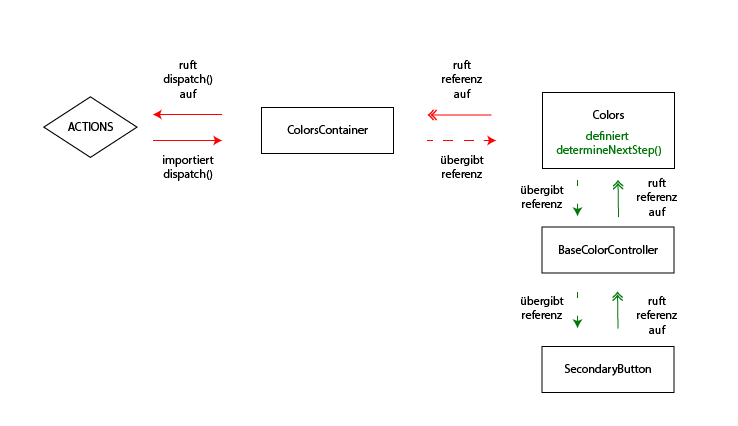
\includegraphics[width=1\textwidth]{images/redux_store_flow.png}
    \caption{Übergabe der \texttt{dispatch()} Methode als Referenz}
    \label{fig:redux_flow}
\end{figure}

In der Komponente \textit{ColorsContainer} wir die Referenz auf die \texttt{dispatch()} Methode als \texttt{prop} mit dem Namen \texttt{setBaseColors} an die Komponente \textit{Colors} übergeben.

Die Komponente \textit{Colors} implementiert die Funktion \texttt{determineNextStep}, die definiert, welcher Schritt in Abhängigkeit vom Entwicklungsziel des Nutzers der Nächste ist, der angezeigt werden soll. Die Referenz auf \texttt{setBaseColors} wird dabei auf jeden Fall aufgerufen. Die Komponente \textit{Colors} gibt nun eine Referenz auf die Funktion \texttt{determineNextStep} an die Komponente \textit{BaseColorController} weiter. Diese wiederum gibt diese Referenz an die Komponente \textit{SecondaryButton} weiter, die die Komponente darstellt, mit der der Nutzer interagiert.

Die \textit{SecondaryButton} Komponente ruft auf einen Klick hin die ihr als \texttt{prop} übergebene Referenz auf eine Funktion auf (siehe Listing \ref{lst:sec_btn}) und hat selbst kein Wissen darüber, welche Funktion innerhalb der Anwendung sie ausführt. Hierdurch werden die übergebenen Referenzen in rückläufiger Reihenfolge wieder aufgerufen und so der \texttt{dispatch()} ausgelöst.

\begin{lstlisting}[caption={Aufruf der übergebenen Funktion in der Komponente \textit{SecondaryButton}}, label=lst:sec_btn]
  function SecondaryButton(props) {
    return (
      <button
        className={setStyles(props.variant, props.inactive)}
        onClick={props.inactive ? '' : props.onClick}
      >
        <SpacingSquishedInset size='l'>
          {props.children}
        </SpacingSquishedInset>
      </button>
    )
}
\end{lstlisting}

\section{CSS-Architektur}
In der Entwicklung von Webanwendungen wird es als gutes Vorgehen angesehen, Inhalte und deren Gestaltung voneinander zu trennen \cite[S. 56]{goodman2002dynamic}. Diese Trennung erfolgt in der Regel durch das Definieren von dedizierten HTML- und CSS-Dateien, die sich nur mit der Struktur von Inhalten bzw. deren Aussehen befassen.
Eine der aktuell verbreitetsten Möglichkeiten, Regeln für die Darstellung von Inhalten zu definieren, ist das Vergeben von Klassen über das \texttt{class}-attribut, die dann in der CSS-Datei über einen Selektor (zum Beispiel \texttt{.myClass}) aufgerufen werden können.

Auch React.js bietet die Möglichkeit, diese Architektur abzubilden. In Kapitel \ref{chap:jsx} wurde bereits erwähnt, dass hier wegen der Verwendung von JavaScript in Komponenten das Attribut \texttt{className} verwendet werden muss.

Durch die Verwendung einer solchen Architektur werden für Komponenten jedoch Abhängigkeiten geschaffen, da für die korrekte Darstellung der Komponente auch immer die entsprechenden Regeln in der CSS-Datei verfügbar sein müssen.
Diese Abhängig von ihrer Umwelt ist jedoch nicht konform mit den in Kapitel \ref{chap:component} definierten Anforderungen an eine Komponente innerhalb dieser Arbeit.

Um das Aussehen innerhalb von HTML-Elementen zu verändern, kann das \texttt{style}-attribut verwendet werden. Auch dieses akzeptiert CSS-Syntax, die das Aussehen des jeweiligen Elements definiert.
React.js ermöglicht die Verwendung dieses Attributes innerhalb von Komponenten und somit auch die Deklaration von Inhalt und Aussehen innerhalb einer Komponente, ohne die Notwendigkeit weiterer Abhängigkeiten.

Die Verwendung des \texttt{style}-attributes zum Festlegen des Aussehens birgt jedoch einige Nachteile. So können über das Attribut keine Pseudo-Klassen, wie zum Beispiel \texttt{:hover} oder \texttt{:before} angesprochen werden. \cite{w3c2017styles}
Für die Entwicklung der Anwendung sind die Pseudo-Klassen jedoch notwendig.
Um dieses Problem zu lösen, wurden im Bereich der \textit{JavaScript-SPAs} viele Bibliotheken entwickelt. Im Rahmen dieses Projektes wurde die Bibliothek Aphrodite\footnotemark{} verwendet.
Diese Bibliothek erlaubt eine Notation der CSS-Regeln wie sie React.js auch nativ ermöglicht, unterstützt aber beispielsweise Pseudo-Klassen (Listing \ref{lst:aphro} zeigt ein simples Beispiel).

\footnotetext{\url{https://github.com/Khan/aphrodite}, zuletzt abgerufen am 12.08.2017}

\begin{lstlisting}[caption=Beipspielhafte Verwendung der Bibliothek Aphrodite, label=lst:aphro]
	import React from 'react'
	import { StyleSheet, css } from 'aphrodite'

	function myComponent(props) {
		<div className={css(styles.componentStyles)} >
			{props.children}
		</div>

		const styles = StyleSheet.create({
			componentStyles: {
				color: 'blue',
				':hover': {
					color: 'red'
			}
		})
	}
\end{lstlisting}

Während der Entwicklung wurde nicht jegliche Art von Gestaltung innerhalb von Komponenten realisiert. Verschiedene native HTML-Elemente, die über die Anwendung hinweg verwendet werden, wurden in einer globalen CSS-Datei definiert. Dies hat den Vorteil, dass zum Beispiel für die Verwendung einer Überschrift keine eigene Komponente geschrieben werden muss, die funktional äquivalent zu einem nativen HTML-Element (beispielsweise \texttt{<h1>}) ist, nur um dessen Aussehen anzupassen.

\section{Interessante Aspekte in der Entwicklung}
Nachfolgend sollen einige konkrete Beispiele aus der Entwicklung der Anwendung erläutert werden. Die verschiedenen Beispiele wurden dabei aus unterschiedlichen Gründen gewählt:
Kapitel \ref{chap:state_component} zeigt einen zentralen Aspekt der Umsetzung einer komponentenbasierten Anwendung mit React.js, Kapitel \ref{chap:display_scope} eine der zentralen Arbeitsweisen der Anwendung. Die Kapitel \ref{chap:colors_dev} und \ref{chap:pdf} zeigen die Lösung von Problemen, die für die Funktionalität der Anwendung eine hohe Relevanz aufweisen.


\subsection{State in Komponenten}
\label{chap:state_component}
Das Konzept des \textit{state} in React.js wurde bereits in Kapitel \ref{chap:stateless} angesprochen. Hier soll an einem konkreten Beispiel verdeutlicht werden, wie der \textit{state} genutzt werden kann, um auf Nutzereingaben zu reagieren und inwiefern sich der Zustand einer Komponente vom Zustand der gesamten Anwendung unterscheidet.
Als Beispiel wurde die Auswahl des Zielmediums durch den Nutzer im ersten Schritt der Anwendung gewählt, die in mehreren Schritten durchgeführt wird.
Der Ablauf der Interaktion mit der Anwendung sieht dabei wie folgt aus:
Die Anwendung präsentiert dem Nutzer drei Optionen, aus denen dieser wählen kann. Wählt der Nutzer eine der Optionen aus, gibt die Anwendung ihm eine visuelle Rückmeldung über die ausgewählte Option. Ist der Nutzer mit seiner Wahl zufrieden, bestätigt er diese durch einen Button und  ihm wir der nächste Schritt im Wizard angezeigt.

Für diese Interaktion werden verschiedene Komponenten eingesetzt (siehe dazu Abbildung \ref{fig:components}), von denen die Meisten zustandslos sind, lediglich die Komponente \texttt{SetupProgress}, die in Listing \ref{lst:setup} zu sehen ist\footnotemark{}, verwaltet einen Zustand.

\begin{figure}[h]
    \centering
    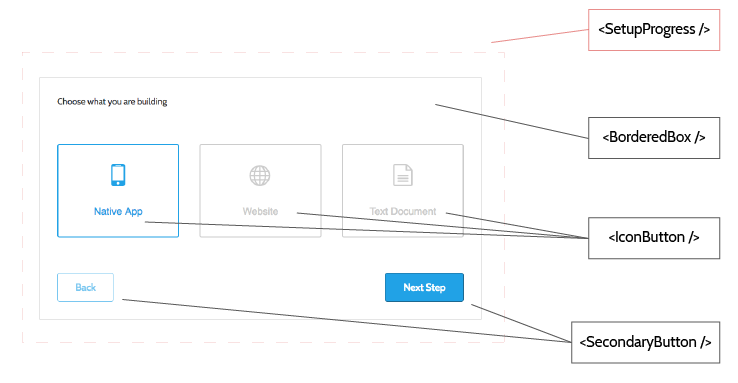
\includegraphics[width=1\textwidth]{images/components.png}
    \caption{Komponenten in der Festlegung des Zielmediums}
    \label{fig:components}
\end{figure}

\footnotetext{Teile des Quellcodes, die für diesen Anwendungsfall nicht relevant sind, wurden gekürzt. Die gesamte Datei kann der beiliegenden CD entnommen werden}

Im \textit{state} der Komponente \texttt{SetupProgress} wird eine Zahl gespeichert die angibt, welche der angezeigten Optionen momentan aktiv ist (ist keine aktiv, wird der Wert auf \texttt{false} gesetzt). Beim rendern der \texttt{IconButton} Komponenten wird für jede Komponente abgeglichen, ob diese im \textit{state} als aktive Option gespeichert ist. Jede der \texttt{IconButton}-Komponenten, die angezeigt wird, ruft über einen Callback die Funktion \texttt{handle\-Icon\-Button\-Click\-(key)} auf, wenn der User auf diese klickt und übergibt einen Key, der wiederum in den \textit{state} der  \texttt{SetupProgress} Komponente geschrieben wird. Durch das Aktualisieren des \textit{state} wird nun die \texttt{render()} Funktion der Komponente erneut aufgerufen und die entsprechende \texttt{IconButton} Komponente wird als aktiv markiert.
Der  \texttt{IconButton} Komponente selbst ist dabei der Kontext, in dem sie verwendet wird, nicht bekannt.


\begin{lstlisting}[caption=Die Komponente \texttt{SetupProgress} in gekürzter Form, label=lst:setup]
  class SetupProgress extends React.Component {
    constructor(props) {
      super(props)

      // Shortened for readability

      this.state = {
        activeOption: false
      }
    }

    handleIconButtonClick(key) {
      this.setState({
        activeOption: key
      })
    }

    handleButtonClick() {
      this.props.setScope(this.state.activeOption)

      // If the current setup step is the last, also set the setup state to finished
      if (this.props.setupStep == this.props.setupSteps) {
        this.props.setSetupToFinished()
      }

      // Reset this components' internal state to disable the button
      this.setState({
        activeOption: false
      })
    }

    handleBackButtonClick() {
      this.props.previousSetupStep()
    }

    /**
     * Generates the main content for the setup component (i.e. Iconbuttons).
     * Determines the correct subset of options and calls constructIconButtons()
     * with that subset.
     *
     * @return {Array} An array of IconButtons ready for rendering
     */
    generateContent() {

      // Shortened for readability

      return this.constructIconButtons(setupOptions)
    }

    /**
     * Constructs an array of IconButtons based on a given set of options
     *
     * NOTE: This will construct an IconButton for every element in the given options
     * and does not validate them.
     *
     * @param {Array} setupOptions
     * @returns {Array} An Array of iconButtons
     */
    constructIconButtons(setupOptions) {
      let iconButtons = []
      for (var i = 0; i < setupOptions.length; i++) {
        let currentOption = setupOptions[i]

        iconButtons.push(
          <div className={css(styles.iconButtonWrapper)}>
            <IconButton
              icon={currentOption.icon}
              onClick={this.handleIconButtonClick}
              key={i}
              identifier={currentOption.value}
              active={this.state.activeOption === currentOption.value}
            >
              {currentOption.text}
            </IconButton>
          </div>

        )
      }

      return iconButtons
    }

    render() {
      return (
        <BorderedBox>
          <SpacingInset size='l'>
            <span>Choose what you are building</span>
            <SpacingInset size='l' />
            <div className={css(styles.buttonWrapperStyles)}>
              {this.generateContent()}
            </div>
            <SpacingInset size='l' />
            <div className={css(styles.buttonWrapperStyles)}>
              <SecondaryButton inactive={this.props.setupStep < 2} onClick={this.handleBackButtonClick} variant={'outline'}>Back</SecondaryButton>
              <SecondaryButton inactive={this.state.activeOption == false} onClick={this.handleButtonClick}>Next Step</SecondaryButton>
            </div>
          </SpacingInset>
        </BorderedBox>
      )
    }
  }

  // Shortened for readability

  export default SetupProgress
\end{lstlisting}

Der hier gezeigte Ablauf hätte sich auch durch die Verwendung des Redux-Stores realisieren lassen, jedoch ist die gewählte Option zunächst nicht für die gesamte Anwendung von Relevanz (so kann der Nutzer seine Auswahl zum Beispiel noch ändern). Erst wenn der Nutzer sich durch den Klick auf den \textit{Next Step} Button auf einen Wert festlegt, wird dieser auch der ganzen Anwendung, über den Redux-Store, bekannt gemacht.

\subsection{Anzeige von Inhalten nach Scope}
\label{chap:display_scope}
Ein Hauptaugenmerk während der Entwicklung lag auf der Anwendung der vom Nutzer gewählten \textit{scopes} in der Anwendung. In Abhängigkeit dieser Scopes muss die Anwendung verschiedene Daten präsentieren. Dabei muss die Möglichkeit bestehen, diese Daten zu erweitern oder zu verändern, ohne dass die Anwendung selbst dafür umstrukturiert werden muss. Diese Datenhaltung soll hier am Beispiel der verschiedenen Schriftfamilien, die im Bereich Typographie Verwendung finden können, gezeigt werden.

Da die Anwendung keine Datenbank implementiert, werden diese Daten in eigenen Dateien als JavaScript-Objekte gespeichert. Listing \ref{lst:fonts_object} zeigt das Objekt, in dem die verschiedenen Schriftarten der \textit{scopes} als Arrays gespeichert sind. Bei Betrachtung des Objektes fällt auf, dass Daten teilweise doppelt auftreten. Obwohl hier gegen das Prinzip \textit{Don’t Repeat Yourself} verstoßen wird, ist eine solche Struktur mit Blick auf eine Weiterentwicklung der Anwendung nötig, um ein möglichst einfaches Verändern eines einzelnen \textit{scopes} gewährleisten zu können.

\begin{lstlisting}[caption=Aufbau des \texttt{FONTS} Objektes, label=lst:fonts_object]
  export const FONTS = {
    DISPLAY: [
      'Verdana', 'Arial', 'Tahoma', 'TrebuchetMS'
    ],
    RESPONSIVE: [
      'Verdana', 'Arial', 'Tahoma', 'TrebuchetMS'
    ],
    NOT_RESPONSIVE: [
      'Verdana', 'Arial', 'Tahoma', 'TrebuchetMS'
    ],
    PAPER_DISPLAY: [
      'Verdana', 'Arial', 'Tahoma', 'TrebuchetMS', 'Times New Roman', 'Georgia', 'Palatino'
    ],
    PAPER: [
      'Times New Roman', 'Georgia', 'Palatino'
    ],
    ANDROID: [
      'Roboto', 'Noto'
    ],
    IOS: [
      'San Francisco'
    ]
  }
\end{lstlisting}

Da die \textit{keys} im \texttt{FONTS} Objekt dabei exakt den möglichen \textit{scopes} entsprechen\footnotemark{}, ist ein einfaches Ermitteln der benötigten Schriftfamilien, wie es in Listing \ref{lst:fonts_access} gezeigt wird, möglich.

\footnotetext{Auch die verschiedenen \textit{scopes} sind konstanten, die in einem Objekt gespeichert werden.}

\begin{lstlisting}[caption=Zugriff auf Werte des \texttt{FONTS} Objektes, label=lst:fonts_access]
  determineFontFamilies() {
    let scope = this.props.scopes[1]
    return FONTS[scope]
  }
\end{lstlisting}

\subsection{Erstellen von Farbkontrasten}
\label{chap:colors_dev}
Die grundlegende Logik zum Errechnen verschiedener Kontrasten wurde bereits im Praxisprojekt definiert. Im ersten Schritt muss die Grundfarbe hierfür in den HSL-Farbraum überführt werden. Für diese Umwandlung wurde in der Anwendung die Bibliothek tinycolor\footnotemark{} verwendet, die verschiedene Funktionen zur Arbeit mit Farben bereit stellt (unter anderem auch das Umwandeln in den HSL-Farbraum).
Nach der Umwandlung in den HSL-Farbraum gibt die Bibliothek ein JavaScript-Objekt zurück, in dem \textit{Hue}, \textit{Saturation}, \textit{Lightness} und \textit{Alpha} als \textit{Key-Value}-Paare vorhanden sind, mit denen die Berechnungen für die Farbkontraste vorgenommen werden können. Die Bibliothek selbst bietet einige Funktionen zum Erstellen von Farbkontrasten, die Ergebnisse dieser Funktionen wurden für den Rahmen dieser Arbeit jedoch als nicht geeignet befunden.

\footnotetext{\url{https://github.com/bgrins/TinyColor}, zuletzt abgerufen am 10.8.2017}

Für einen Komplementär-Kontrast muss der \textit{Hue}-Wert der Grundfarbe um 180° verändert werden. Die Berechnung erwies sich mit Hilfe des HSL-JavaScript-Objektes als recht simpel, hier musste lediglich darauf geachtet werden, den einen Wert von 360 nicht zu überschreiten.
Die Berechnung des triadischen Kontrastes gestaltet sich ähnlich, hier wurde der \textit{Hue}-Wert jedoch um 30° erhöht beziehungsweise verringert, um den gewünschten Effekt zu erzielen.

Deutlich komplexer gestaltet die Generierung von monochromatischen Farbschemata, da die Farben hier in ihrem \textit{Hue}-Wert unverändert bleiben, jedoch in ihrem \textit{Saturation} und/oder ihrem \textit{Lightness}-Wert verändert werden können. Weiterhin werden für dieses Farbschema mehr Farben benötigt (die Anwendung arbeitet mit der Grundfarbe und drei veränderten Farben).

Für jede Farbe müssen hier also verschiedene Entscheidungen getroffen werden. Zunächst muss entscheiden werden, welche Werte verändert werden können. Möglich ist hier einer von drei Fällen:

\begin{itemize}
  \item Nur der \textit{Saturation}-Wert
  \item Nur der \textit{Lightness}-Wert
  \item Sowohl der \textit{Saturation}- als auch der \textit{Lightness}-Wert
\end{itemize}

Um hier dynamischere Ergebnisse liefern zu können, wird diese Entscheidung in der Funktion \texttt{calculateMonochromaticColors}, die Listing \ref{lst:mono} zeigt, zufällig getroffen.

\begin{lstlisting}[caption=Berechnung eines Monochromatischen Farbschemas, label=lst:mono]
  /**
   * Calculates a color scheme of monochromatic colors based on a base color with a variable amount of colors.
   * The colors returned by this function are random in saturation and lightness.
   * The colors returned by this function are guaranteed to not be equal to either each other, nor the base color.
   *
   * NOTE: Since the colors cannot be similar to each other, the amount of options in limited. Therefor, the number of colors to be returned should not be too high (6 will probably still work fine, whereas 25 will cause the function to break.)
   *
   * @param amount The number of colors that should be returned
   * @param baseColor A HEX-Value of a color that is the basis of the color scheme
   * @returns An Array of HEX-Values that build a monochromatic color scheme
   */
  export function calculateMonochromaticColors(amount, baseColor) {

    let hslColor = convertToHsl(baseColor)
    let colors = []

    for (var i = 0; i < amount; i++) {
      let currentColor = Object.assign({}, hslColor)
      let randomOption = CHANGABLE_COLOR_ATTRIBUTES[Math.floor(Math.random() * 3)]
      let changedColor = changeValuesOfColor(randomOption, currentColor)

      // Check, if the color is similar to the base color
      let similarToBaseColor = colorsAreSimilar(hslColor, changedColor)
      while (similarToBaseColor) {
        changedColor = changeValuesOfColor(randomOption, changedColor)
        similarToBaseColor = colorsAreSimilar(hslColor, changedColor)
      }

      if (colors.length < 1) {
        colors.push(convertToHex(changedColor))
      } else {
        // Check, if the new color is similar to other colors that were calculated
        let similarColorsPresent = colorInArrayIsSimilar(colors, changedColor)
        while (similarColorsPresent) {
          changedColor = changeValuesOfColor(randomOption, changedColor)
          similarColorsPresent = colorsAreSimilar(colors, changedColor)
        }
        colors.push(convertToHex(changedColor))
      }
    }

    return colors
  }
\end{lstlisting}

Im nächsten Schritt müssen die Veränderungen in den bestimmten Werten vorgenommen werden, auch hier werden diese Werte zufällig gewählt. Um auszuschließen, dass die definierten Werte zu hell oder zu dunkel (also fast Schwarz oder fast Weiß) sind und damit sehr wenig Farbe aufweisen, wurden die Wertebereiche, in denen \textit{Lightness} und \textit{Saturation} verändert werden können, begrenzt. Dieser Vorgang findet in der Funktion \texttt{changeValuesOfColor} statt (siehe Listing \ref{lst:hsl}).

\begin{lstlisting}[caption=Setzen der HSL-Werte, label=lst:hsl]
  /**
   * Changes the lightness and/or saturation value of an HSL color object to a random value and returns a copy of that object.
   * The random values are restricted to prevent them from beign colorless (i.e. almost black or almost white).
   * A switch case determines, which attribute(s) of the color should be changed.
   *
   * @param attributeToChange The attribute on the color to be changed
   * @param color An HSL color object on which's hue the new color will be based
   * @returns An HSL color object with the manipulated attributes
   */
  function changeValuesOfColor(attributeToChange, color) {
    let manipulatedColor = Object.assign({}, color)
    let lightnessVal = Math.random() * 0.85 + 0.15
    let saturationVal = Math.random() * 0.65 + 0.15

    switch (attributeToChange) {
      case 'LIGHTNESS':
        manipulatedColor.l = lightnessVal.toFixed(2)
        break
      case 'SATURATION':
        manipulatedColor.s = saturationVal.toFixed(2)
        break
      case 'LIGHTNESS_SATURATION':
        manipulatedColor.l = lightnessVal.toFixed(2)
        manipulatedColor.s = saturationVal.toFixed(2)
        break
      default:
        throw new 'Oops, seems like the randomizer messed something up.'
    }

    return manipulatedColor
  }
\end{lstlisting}

Nachdem die Farben festgelegt sind muss außerdem überprüft werden, ob  eine generierte Farbe a) zu ähnlich der Grundfarbe oder b) zu ähnlich einer anderen generierten Farbe ist.
Als \textit{zu ähnlich} zueinander wurden hier zwei Farben definiert, der \textit{Saturation}- \textbf{und} \textit{Lightness}-Werte eine Differenz kleiner als 0.1 aufweisen. Farben, die nur in einem der beiden Werte eine zu kleine Differenz aufweisen, werden nicht als zu ähnlich verstanden.
Die Ähnlichkeit zweier Farben wird in  der Funktion \texttt{colorsAreSimilar} in Listing \ref{lst:similar} deutlich. Die Funktion gibt dabei \texttt{true} zurück, wenn die beiden übergebenen Werte zu ähnlich sind. Anstatt der betroffenen Farbe wird dann in der Funktion \texttt{calculateMonochromaticColors} eine neue generiert.

\begin{lstlisting}[caption=Überprüfen der Ähnlichkeit zweier Farben, label=lst:similar]
  /**
   * Checks if two HSL color objects are similar.
   * Similarity is defined as the Lightness and Saturation being less than 0.1 apart,
   * with the Hue being exactly the same.
   *
   * NOTE: The Hue of the colors is not taken into consideration.
   *
   * @param color The first HSL color object
   * @param candidate The second HSL color object
   * @returns true if the two colors are found to be similar
   */
  function colorsAreSimilar(color, candidate) {
    let saturationDifference = Math.abs(color.s - candidate.s)
    let lightnessDifference = Math.abs(color.l - candidate.l)

    if (saturationDifference < 0.1 && lightnessDifference < 0.1) {
      return true
    }

    return false
  }
\end{lstlisting}


\subsection{Erstellen von PDF-Dateien}
\label{chap:pdf}
Wie in Kapitel \ref{chap:results} bereits angesprochen, soll dem Nutzer im letzten Schritt der Anwendung, neben der einfachen Darstellung, die Möglichkeit gegeben werden, seine Ergebnisse in Form einer PDF-Datei zu speichern.\\
Für die Generierung einer PDF-Datei bieten sich verschiedene Möglichkeiten. Da in der Anwendung kein Backend enthalten ist, können Lösungen, die einer Serverseitige Generierung von PDF-Dateien implementieren, bereits zu Beginn ausgeschlossen werden.\\

Eine der simpelsten Möglichkeiten, eine PDF-Datei nutzerseitig zu erzeugen, ist ein Drucken als PDF Datei über das Betriebssystem des Nutzers. Hierbei müsste für die Seite lediglich ein entsprechendes Stylesheet hinterlegt werden, welches das Layout gegebenenfalls für den Druck anpasst. Diese Lösung weist allerdings eine beschränkte Verfügbarkeit auf: Das Betriebssystem macOS bieten den Druck als PDF beispielsweise nativ an, das Betriebssystem Windows aber erst seit der neusten Version, Windows 10. Somit könnte diese Funktion nicht von allen Nutzer verwendet werden.\\

Eine weitere Möglichkeit stellt die Bibliothek html2canvas\footnotemark{} dar. Die Bibliothek erlaubt das Speichern von Seiten als Bilddateien. Die Verfügbarkeit ist hier deutlich höher als beim Drucken als PDF, jedoch bringt das Speichern als Bild einige Restriktionen mit sich. So können beispielsweise Werte in der Datei nicht markiert und kopiert werden, was einen erhöhten Arbeitsaufwand für den Nutzer bedeutet.

\footnotetext{\url{https://github.com/niklasvh/html2canvas}}

Die Entscheidung viel aus diesen Gründen auf die Bibliothek jsPDF\footnotemark{}. Diese erlaubt das Erstellen von PDF-Dateien im Browser und auch das Einfügen von DOM-Elementen in PDF-Dateien.
Das Einfügen von DOM-Elementen ist zwar komfortabel, bedeutet aber auch einen (zumindest teilweisen) Verlust der Kontrolle über die Struktur und das Aussehen der PDF-Datei.
Aus diesem Grund wurde die Möglichkeit für die manuelle Erzeugung von PDF-Dateien genutzt, die die Bibliothek ebenfalls ermöglicht. Hierfür steht eine API zur Verfügung, mit der verschiedene Elemente (wie Text oder geometrische Formen), unter Angabe der Position auf der x- und y-Achse, in die Datei eingefügt werden können. Listing \ref{lst:pdf} zeigt eine gekürzte Version der Funktion, die die PDF-Datei erzeugt und speichert, Abbildung \ref{fig:pdf} eine beispielhafte PDF-Datei, die von der Anwendung erstellt wurde.

\begin{lstlisting}[caption={Beispilehafte Generierung einer PDF-Datei}, label=lst:pdf]
  export function generatePDF(typography, colors) {
    var pdf = new pdfConverter('p', 'mm', 'a4')

    // shortened for readability

    pdf.addImage(imgData, 'PNG', 65, 10, 81, 30)
    pdf.setFontSize(10)
    pdf.text('These are the values you gathered with the help of 25knots', 10, 50)

    pdf.setFontSize(20)
    pdf.text('Typography', 10, 70)
    pdf.setFontSize(10)
    pdf.text('Font Family:', 10, 80)
    pdf.text(typography.general.fontFamily, 50, 80)

    // shortened for readability

    let date = new Date()
    let dateString = date.getFullYear() + '-' + (date.getMonth() + 1 ) + '-' + date.getDate() + '-' + date.getHours() + '-' + date.getMinutes()
    pdf.save('25knots_' + dateString + '.pdf')
  }
\end{lstlisting}

\footnotetext{\url{https://github.com/MrRio/jsPDF}}

Für den aktuellen Umfang der Anwendung ist diese Lösung praktikabel, bei einer Erweiterung des Funktionsumfangs muss diese Methode jedoch erneut, auf das Verhältnis von Aufwand und Nutzen hin evaluiert werden

Um dem Nutzer eine spätere Zuordnung der Datei zu vereinfachen, wird diese im Namen mit dem aktuellen Datum und der Uhrzeit versehen. Eine bessere Möglichkeit wäre, es dem Nutzer zu ermöglichen, sein Projekt zu beginn der Benutzung der Anwendung zu benennen.

\begin{figure}[h]
    \centering
    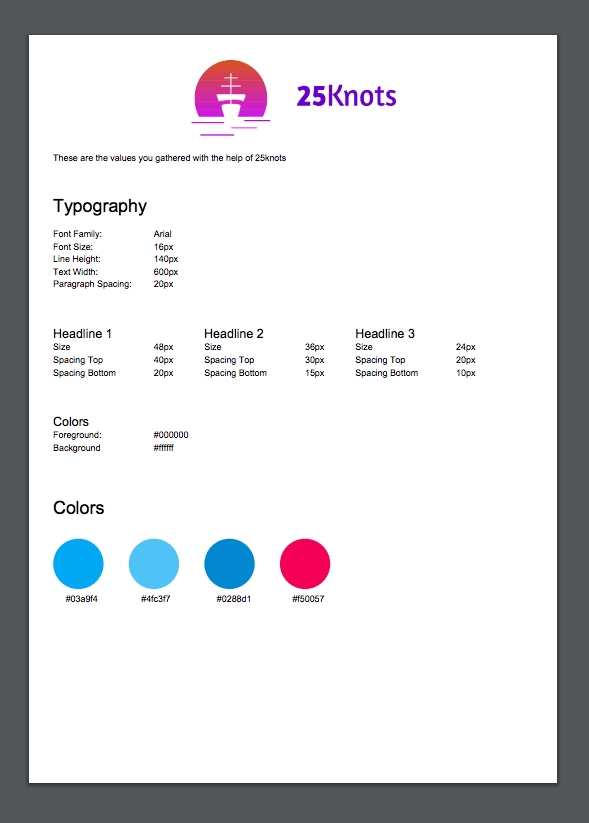
\includegraphics[width=0.4\textwidth]{images/pdf_generated.png}
    \caption{Beispiel einer generierten PDF-Datei}
    \label{fig:pdf}
\end{figure}

\chapter{Veröffentlichung der Anwendung}
\thispagestyle{fancy}

Bei der Textgestaltung und automatischen Änderung von Abbildungsnummern, Querverweisen,
Seitenzahlen, Gliederungen, Literaturhinweisen etc. bietet sich der Rückgriff
auf moderne Textverarbeitungsprogramme an. Nutzen Sie diese zur besseren Lesbarkeit
und Strukturierung des Textes, aber vermeiden Sie überflüssige Spielereien. Da
besonders bei Textdokumenten mit eingebundenen Objekten wie Bildern, Formeln

\section{Hosting}
Um den Zugang zur Anwendung für die Community möglichst einfach zu gestalten, bietet es sich an, diese zu hosten (einer andere, weniger geeignete Möglichkeit, wäre beispielsweise nur die Veröffentlichung des Quellcodes und das lokale hosten durch den Nutzer selbst).
Da es sich bei der Anwendung um eine rein Clientseitige handelt, stehen eine Vielzahl von Möglichkeiten für das hosting zu Verfügung, da der Server lediglich statische html- und JavaScript-Dateien ausliefern muss.

In die nähere Auswahl kamen in diesem Projekt Github Pages und Heroku. Ein hosting auf einem privaten Server wurde schnell ausgeschlossen, um die mögliche zusätzliche Arbeit möglichst gering zu halten.
Da der Quellcode der Anwendung bereits auf Github veröffentlich wurde, scheint das Hosting über Github Pages zunächst die naheliegendste und einfachste Lösung. Ein Deployment auf Github Pages erfolgt nach entsprechenden Einstellungen im Repository einfach durch einen push auf den gh-pages branch. Die Anwenudung ist danach über die Domain username.github.io/rpository erreichbar. Größter Vorteil ist dabei, dass kein externer Service benötigt wird. Es treten aber auch einige Limitierungen auf. Beim testen der Hosting-Möglichkeiten wurde deutlich, dass das Modul React-Router den zusätzlichen Path nicht ohne weiteres unterstützt. Zwar bieten sich hier relative einfach Lösungen wie das verwenden von hashes anstatt von Pfaden im React-Router an, jedoch wurde mit blick auf die bereits bei simplen dingen auftretenden Probleme diese Möglichkeit zunächst als weniger geeignet eingestuft.

Für das Hosting wurde sich für den Service Heroku entschieden. Heroku ist ein Saas, das ein Deployment und hosting ohne Setup und Konfiguration erlaubt. Ein Deployment auf Heroku läuft dabei über einen remote branch im git repository, kann also mit dem Befehl \verb|git push heroku master| gestartet werden. Heroku erkennt die verwendete Sprache automatisch und stellt alles nötige automatisch ein.
Jedoch unterstützt Heroku lediglich Serverseitige Progrmmiersprachen und beitet keinen Support für das Hosting von statischen files. Um diese Anwendung zu hosten, muss also ein Server geschreiben werden. Da dieser nur statische Files hosten muss, ist dieser sehr simple in Node.js und dem Framework express geschrieben:

\begin{lstlisting}
  const express = require('express')
  const app = express()

  app.use(express.static(__dirname + '/dist'))
  app.listen(process.env.PORT || 8080)
\end{lstlisting}

Der Server hostet dabei den ordner \verb|dist|, in dem sich die gebuildeten Files befinden (unter anderem auch die Datei \verb|index.html|, auf die ein Browser automatisch zurück greift). Mit der Datei \verb|Procfile| wird Heroku dann mitgeteilt, welche Befehle beim Deployment der Anwendung ausgeführt werden soll. Im Falles dieser Anwendung ist das die Datei \verb|server.js|. Das \verb|Procfile| besteht alsolediglich aus der Zeile

\begin{lstlisting}
  web: node server.js
\end{lstlisting}

Da sowohl Github Pages, als auch Heroku von sich aus eine recht kryptische URL verwenden, wurde weiterhin die Domain \verb|25knots.de| gekauft, um auch hier den Einstieg für potentielle Nutzer so einfach wie möglich zu gestalten.


\section{Weiterentwicklung}
Nachfolgend soll außerdem auf eine mögliche Weiterentwicklung der Anwendung nach dem Abschluss dieser Arbeit eingegangen werden. In diesem Zusammenhang stellen sich vor allem drei Fragen:
\begin{enumerate}
  \item Wie können Personen aus der Community dazu gebracht werden, an einer Weiterentwicklung mitzuarbeiten?
  \item Wie kann eine durchgängig hohe Qualität des Quellcodes garantiert werden, auch wenn viele verschiedene Menschen daran arbeiten?
  \item Wie kann das Mitwirken für Interessenten möglichst einfach gestaltet werden?
\end{enumerate}

Eine konkrete Beantwortung der ersten Frage gestaltet sich recht schwierig. Es lässt sich jedoch ein logischer Zusammenhang zwischen der Anzahl der Nutzer und der Anzahl der Mitwirkenden eines Projektes feststellen. Am Beispiel der Plattform Github können \textit{stars} als relativ sichere Mindestzahl der Nutzer gesehen werden. Laut \cite{borges2015popularity} besteht ein Zusammenhang zwischen \textit{stars} und der anzahl der Mitwirkenden an einem Projekt:

\begin{quote}
  In git-based systems, forks are used to either propose changes to an application or as
a starting point for a new project. In both cases, the number of forks can be seen as a proxy
for the importance of a project in GitHub. [...] Two facts can be observed in this figure. First, there is a strong positive
correlation between stars and forks (Spearman rank correlation coefficient = 0.55). Second,
only a few systems have more forks than stars.
\end{quote}

Somit ist eine Steigerung der Mitwirkenden also automatisch mit einer Steigerung der Nutzer der Anwendung verbunden. Der Inhalt diese Abschnittes soll also vorrangig mit der Beantwortung der zweiten und dritten Frage beschäftigen.

\subsection{Sicherung der Code-Qualität}
zahlen, Gliederungen, Literaturhinweisen etc. bietet sich der Rückgriff
auf moderne Textverarbeitungsprogramme an. Nutzen Sie diese zur besseren Lesbarkeit
und Strukturierung des Textes, aber vermeiden Sie überflüssige Spielereien. Da
besonders bei Textdokumenten mit eingebundenen Objekten wie Bildern, Formeln

\subsection{Dokumentation}
zahlen, Gliederungen, Literaturhinweisen etc. bietet sich der Rückgriff
auf moderne Textverarbeitungsprogramme an. Nutzen Sie diese zur besseren Lesbarkeit
und Strukturierung des Textes, aber vermeiden Sie überflüssige Spielereien. Da
besonders bei Textdokumenten mit eingebundenen Objekten wie Bildern, Formeln

\subsection{Contribution Guidelines}
zahlen, Gliederungen, Literaturhinweisen etc. bietet sich der Rückgriff
auf moderne Textverarbeitungsprogramme an. Nutzen Sie diese zur besseren Lesbarkeit
und Strukturierung des Textes, aber vermeiden Sie überflüssige Spielereien. Da
besonders bei Textdokumenten mit eingebundenen Objekten wie Bildern, Formeln

\subsection{Tests}
zahlen, Gliederungen, Literaturhinweisen etc. bietet sich der Rückgriff
auf moderne Textverarbeitungsprogramme an. Nutzen Sie diese zur besseren Lesbarkeit
und Strukturierung des Textes, aber vermeiden Sie überflüssige Spielereien. Da
besonders bei Textdokumenten mit eingebundenen Objekten wie Bildern, Formeln

\section{Vermarktung}
Bei der Textgestaltung und automatischen Änderung von Abbildungsnummern, Querverweisen,
Seitenzahlen, Gliederungen, Literaturhinweisen etc. bietet sich der Rückgriff
auf moderne Textverarbeitungsprogramme an. Nutzen Sie diese zur besseren Lesbarkeit
und Strukturierung des Textes, aber vermeiden Sie überflüssige Spielereien. Da
besonders bei Textdokumenten mit eingebundenen Objekten wie Bildern, Formeln

\chapter{Fazit \& Ausblick}
\thispagestyle{fancy}

Bei der Textgestaltung und automatischen Änderung von Abbildungsnummern, Querverweisen,
Seitenzahlen, Gliederungen, Literaturhinweisen etc. bietet sich der Rückgriff
auf moderne Textverarbeitungsprogramme an. Nutzen Sie diese zur besseren Lesbarkeit
und Strukturierung des Textes, aber vermeiden Sie überflüssige Spielereien. Da
besonders bei Textdokumenten mit eingebundenen Objekten wie Bildern, Formeln

\section{Zielerreichungsgrad}
Zunächst lässt sich feststellen, dass im Rahmen der vorliegenden Arbeit eine Anwendung Konzipiert, Gestaltet und Umgesetzt werden konnte, die nach den in Kapitel 1 definierten Maßstäben eine Marktfähige Anwendung ist.
Die Anwendung biete, sowohl durch ihre Gestaltung, als auch durch ihre Programmierung eine befriedigende Nutzererfahrung. Dem Nutzer gegenüber wird deutlich kommuniziert, an welchem Punkt der Anwendung er sich befindet und er erhält einen Mehrwert aus der Verwendung der Anwendung.
Durch das Hosting und die damit verbunden Domain ist die Anwendung weiterhin für Nutzer leicht zugänglich. Außerdem ist sie auch für Nutzer, die an einer Mitarbeit an der Anwendung interessiert sind durch das öffentliche Repository und die darin erläuterten Wege zur Mitarbeit leicht zugänglich.
Weiterhin ist die Anwendung eine ersten Gruppe von Personen bekannt. Hier fällt es schwer, den Grad der Zielerreichung festzulegen, da es sich zum Einen schwierig gestaltet, die Bekanntheit zu messen, die Bekanntmachung der Anwendung zum Anderen aber auch ein andauernder Prozess ist.

Auch die Mitarbeit an der Anwendung durch die Community lässt sich zu diesem Zeitpunkt noch nicht beurteilen, da die Anwendung etwa Zeitgleich mit Fertigstellung dieser Arbeit veröffentlicht wurde. Es lässt sich jedoch feststellen, dass die Grundsteine für eine mögliche Mitarbeit von anderen gelegt wurden.

An dieser Stelle sei außerdem noch einmal der geplante Umfang der Anwendung angesprochen. Hier wurde der Bereich “Layouts \& Grid” zwar zu beginn als wünschenswert definiert, jedoch konnte dieser in der ersten Version der Anwendung (wie in Kapitel 3.6 ausgeführt) nicht implementiert werden. Dies ist vor dem Gedanken, dass hier ein MVP erstellt werden sollte jedoch hinnehmbar.

\section{Ausblick}
Wie bei der Entwicklung jeder Anwendung ist es auch hier schwer, an einem bestimmten Punk von einer “fertigen Anwendung” zu sprechen. Es konnte eine Anwendung erstellt werden, die gemessen am Rahmen der Arbeit und dem vorgegebenen Arbeitsaufwand als fertig bezeichnet werden kann. Für sich betrachtet, bieten sich noch viele Möglichkeiten, die Anwendung zu erweitern und in ihrem aktuellen Stand zu verbessern.
Einige potentielle Verbesserungen des aktuellen Standes wurden bereits in den zugehörigen Kapiteln angesprochen. Diese wurden als Issues mit in der Github Repository übernommen, um so bereits erste Schritte für die Weiterentwicklung zu gehen.

Weiterhin bieten sich Erweiterungen der Anwendung in From von neuen Themengebieten an. Diese können die in Kapitel 1 definierten sein, jedoch können durchaus auch komplett neue, noch gar nicht bedachte Themengebiete auftreten.
Ein weiterer, interessanter Punkt ist die intensivere Nutzung der Scopes. Diese haben momentan nur sehr subtile Auswirkungen, für jeden Anwendungsfall durchläuft der Nutzer jedoch die gleiche Anwendung, die sich nur in Details unterscheidet. Mit weiteren Anwendungsgebieten kann auch hier eine erhöhte diveristät der verschiedenen Scopes angenommen werden.

Generell lässt sich die Wahl von React.js zur Umsetzung der Anwendung auch weiterhin vertreten. Die Library bietet zum einen die nötigen Möglichkeiten zur Erweiterung der Anwendung, zum anderen aber auch das Potential, auf Dauer als interessantes Projekt zu wirken.


\section{Fazit}
Für mich persönlich war die Arbeit an dem Projekt im Rahmen dieser Arbeit sehr spannend. Hier konnte ich viele Rollen bekleiden, die in einem größeren Projekt wahrscheinlich von verschiedenen Personen bekleidet werden und so die verschiedenen Aufgabenbereiche kennen lernen.
Das Ökosystem um React.js war dabei ein sehr spannendens. Man merkt diesem das Junge alter der Library dabei an. Viele Best Practices ändern sich häufig und sind nicht so sehr verinnerlicht wie in anderen, älteren Libraries wie beispielsweise Ruby on Rails. Häufig kann man dabei mitverfolgen, wie sich best practices im Rahmen von Diskussionen auf Seiten wie Github herausstellen. Weiterhin werden recht häufig neue Versionen von Bibliotheken veröffentlicht, die dafür sorgen, dass das Ökosystem sehr lebendig bleibt.

Neu war für mich persönlich auch die Situation, ein Produkt mit dem Hintergedanken zu entwickeln, dass dieses nicht nur jemand nutzen soll, sondern auch jemand komplett fremdes Einblick in den Code bekommen und an diesem mitarbeiten könnte.

Insgesamt war die Arbeit an diesem Projekt eine sehr spannende, die sicherlich auch außerhalb des Rahmens dieser Arbeit noch weiter gehen wird.

[ HIER VIELLEICHT NOCH COOLES ZITAT ]


%Erzeugt das Literaturverzeichnis anhand der Datei "`literatur.bib"'
\bibliographystyle{alpha}
\bibliography{bibliography}
\end{document}
